% MIT Coding Challenge — Final Writeup
% Figure-driven narrative with tables/figures at end
\documentclass[12pt]{article}
\usepackage[margin=1in]{geometry}
\usepackage{amsmath,amssymb}
\usepackage{graphicx}
\usepackage{booktabs}
\usepackage{natbib}
\usepackage{hyperref}
\usepackage{float}
\usepackage{caption}
\usepackage{subcaption}
\usepackage{setspace}
\usepackage{appendix}
\onehalfspacing

% For end-of-document floats
\usepackage[nomarkers,nolists]{endfloat}
\renewcommand{\efloatseparator}{\mbox{}}

\title{U.S. Monetary Policy Spillovers to Exchange Rates:\\
Evidence from High-Frequency Identification}
\author{Trenton Eugene O'Bannon\\MIT Coding Challenge Submission}
\date{\today}

\begin{document}

\maketitle

\begin{abstract}
I examine the transmission of U.S. monetary policy surprises to G10 exchange rates using high-frequency identification. Combining federal funds futures surprises with daily spot exchange rates for eight currencies (1994--2024), I document three findings. First, U.S. Treasury yields respond strongly to monetary policy surprises, validating the identification strategy. Second, daily exchange rate responses are heterogeneous and imprecisely estimated, with $R^2$ values below 1\%. Third, cross-country net foreign asset positions (NFA/GDP) do not robustly explain heterogeneity in FX responses---neither unconditionally, post-2008, nor during high-volatility episodes. These null results do not reject the theoretical relevance of balance-sheet channels; rather, they indicate that within a G10 daily-frequency event-study design, net external positions are not a sufficient statistic for currency exposure to U.S. monetary shocks.
\end{abstract}

\newpage
\tableofcontents
\newpage

%==============================================================================
\section{Introduction}
%==============================================================================

Understanding how U.S. monetary policy transmits to international asset prices is central to open-economy macroeconomics. The Federal Reserve's policy decisions affect global financial conditions through multiple channels: interest rate differentials, portfolio rebalancing, risk premia, and valuation effects on dollar-denominated assets \citep{rey2015dilemma, bruno2015cross}.

This paper uses high-frequency identification to isolate exogenous monetary policy surprises and trace their effects on G10 exchange rates. Following \citet{bauer2023reassessment}, I decompose FOMC announcement effects into target rate surprises (MP1) and forward guidance/statement surprises (STMT). I then test a specific mechanism: whether cross-country differences in external balance sheet positions---measured by net foreign assets relative to GDP---explain heterogeneity in exchange rate responses, as suggested by \citet{antolin2023advances}.

\textbf{Why this matters}: The balance-sheet channel is central to modern international macro-finance. If countries with larger dollar liabilities (negative NFA) experience larger depreciations on Fed tightening, this has implications for global financial stability, optimal reserve holdings, and the international monetary system. Testing this mechanism in clean high-frequency data disciplines the growing literature on dollar dominance and U.S. policy spillovers \citep{gopinath2020dominant}.

The empirical strategy proceeds in four steps:
\begin{enumerate}
    \item \textbf{Shock construction and validation} (Section~\ref{sec:validation}): I document the time-series properties of monetary surprises and validate them against Treasury yield responses.
    \item \textbf{Asset price responses} (Section~\ref{sec:responses}): I estimate the effects on yields and FX, establishing that yields respond strongly while FX responses are noisy.
    \item \textbf{Balance-sheet mechanism} (Section~\ref{sec:mechanism}): I test whether NFA/GDP explains cross-country heterogeneity in FX responses.
    \item \textbf{Regime variation} (Section~\ref{sec:regimes}): I test whether the NFA channel strengthens post-GFC or during high-VIX stress episodes.
\end{enumerate}

The main findings are: (i) Treasury yields respond approximately 1.0 basis points per 1 basis point STMT surprise, validating identification; (ii) FX responses are heterogeneous but imprecisely estimated ($R^2 < 0.01$); (iii) NFA/GDP does not robustly mediate FX responses in any specification. These null results are informative, not discouraging: they imply that \textbf{in advanced economies, net external positions are not a sufficient statistic for currency exposure to U.S. monetary shocks at daily frequency}. This disciplines the mechanism---if balance-sheet effects operate in G10, they require gross currency mismatch data or longer horizons to detect.

%==============================================================================
\section{Data and Methodology}
%==============================================================================

\subsection{Monetary Policy Surprises}

I use high-frequency surprises constructed from federal funds futures prices in narrow windows around FOMC announcements \citep{bauer2023reassessment}. Because realized policy decisions respond endogenously to macroeconomic conditions, event-study identification isolates the \textit{unexpected} component of policy, following the approach of Kuttner (2001) and Nakamura--Steinsson (2018).

The key measures are:
\begin{itemize}
    \item \textbf{MP1}: The surprise change in the current-month federal funds futures rate, capturing unexpected target rate changes.
    \item \textbf{STMT}: A statement/principal-component surprise aggregating information across short-rate instruments, capturing both target and forward-guidance news.
\end{itemize}

I focus on STMT as the baseline shock because it summarizes both dimensions of monetary news in a single series with interpretable units. MP1 serves as a robustness measure focusing narrowly on target rate surprises. Table~\ref{tab:surprise_summary} presents summary statistics.

\subsection{Exchange Rate Data}

Daily spot exchange rates for eight G10 currencies: AUD, CAD, CHF, EUR, GBP, JPY, MXN, and NOK. I express rates as foreign currency per USD (e.g., JPY/USD = 150).

\textbf{Convention}: The dependent variable is the spot return:
\begin{equation}
r_{i,t} = -\Delta\log(e_{i,t})
\end{equation}
where $e_{i,t}$ is foreign currency per USD. Under this convention, $r > 0$ indicates foreign appreciation (USD depreciation). This matches \citet{antolin2023advances}, ensuring coefficient signs are directly comparable.

\subsection{Net Foreign Asset Data}

Country-level NFA/GDP comes from the External Wealth of Nations database \citep{lane2018external}. I use lagged annual values to avoid reverse causality. Table~\ref{tab:nfa_summary} shows substantial cross-sectional variation: Switzerland (+142\% GDP) and Norway (+68\%) are large creditors; Mexico ($-39\%$) and Australia ($-52\%$) are debtors.

\subsection{Inference}

Following \citet{petersen2009estimating}, I cluster standard errors by FOMC date to account for the common shock structure: the monetary surprise is identical across currencies on each announcement day. This is the appropriate clustering dimension when the regressor of interest (STMT or MP1) varies only at the time level.

%==============================================================================
\section{Shock Construction and Validation}
\label{sec:validation}
%==============================================================================

Before examining exchange rate responses, I validate that the monetary policy surprises capture meaningful policy news.

\subsection{Time-Series Behavior and Regime Variation}

Figure~\ref{fig:surprise_timeseries} shows the STMT series over time. Large negative surprises concentrate in crisis episodes (2008--2009 and 2020), consistent with unexpectedly aggressive easing. The 2022--2024 tightening period features frequent positive surprises. This time variation implies that identification is driven by distinct monetary regimes---crisis easing, ZLB/forward guidance, and tightening cycles---motivating later regime-split tests.

Figure~\ref{fig:surprise_correlation} shows that STMT correlates highly with both MP1 (target surprise) and MP2 (path surprise), indicating it loads on multiple dimensions of monetary news rather than isolating a single component. This supports using STMT as a summary shock while reserving MP1 for robustness.

\subsection{Distributional Properties}

Figure~\ref{fig:surprise_distribution} shows that surprise measures have means near zero, consistent with market efficiency. However, the distributions exhibit fat tails: a small number of extreme events (crisis announcements) contribute disproportionately to identification. These tails are important for inference---outliers can influence slope estimates---but they also reflect genuine policy variation.

\subsection{External Validation: Treasury Yields}

Despite being constructed from futures-rate instruments, STMT should comove with Treasury yields on FOMC days if it captures policy-relevant news. Figure~\ref{fig:stmt_validation} confirms this: the scatter of STMT against 2-year and 10-year yield changes shows a tight positive relationship, indicating that the shock moves the yield curve as expected.

\subsection{Regime-Dependent Volatility}

Figure~\ref{fig:volatility_regimes} shows that surprise volatility is substantially higher in crisis periods than in normal regimes. This heteroskedasticity reinforces the motivation for regime interactions: if transmission channels differ in stress versus calm periods, coefficient estimates may mask this heterogeneity unless we condition on regime.

%==============================================================================
\section{Asset Price Responses}
\label{sec:responses}
%==============================================================================

\subsection{Treasury Yields: Strong, Systematic Response}

I estimate:
\begin{equation}
\Delta y_{\tau,t} = \alpha + \beta \cdot \text{STMT}_t + \varepsilon_t
\end{equation}
where $\Delta y_{\tau,t}$ is the $\tau$-maturity Treasury yield change on FOMC date $t$.

Table~\ref{tab:treasury_response} reports results. A 1 basis point STMT surprise raises the 2-year yield by approximately 1.0 basis points ($R^2 \approx 0.27$). The response declines monotonically with maturity, consistent with monetary surprises primarily shifting near-horizon expected policy rates. Figure~\ref{fig:treasury_coefficients} visualizes this term-structure pattern: the declining response with maturity is the expected signature of conventional transmission.

\textbf{Takeaway}: The yield response validates identification---STMT captures meaningful monetary news. The high $R^2$ relative to daily noise confirms that announcement-day yield changes are largely explained by the surprise.

\subsection{Exchange Rates: Heterogeneous but Noisy}

I estimate currency-by-currency regressions:
\begin{equation}
r_{i,t} = \alpha_i + \beta_i \cdot \text{STMT}_t + \varepsilon_{i,t}
\end{equation}

Table~\ref{tab:fx_response} and Figure~\ref{fig:fx_coefficients} show the results. All coefficients are negative, consistent with theory: hawkish surprises lead to foreign depreciation. However:
\begin{itemize}
    \item No coefficient is individually significant at conventional levels.
    \item $R^2$ values are uniformly low ($< 1\%$), indicating daily FX returns are dominated by non-monetary factors.
    \item There is meaningful dispersion in point estimates across currencies.
\end{itemize}

\textbf{Takeaway}: The contrast with Treasury yields is striking. Figure~\ref{fig:unified_coefficients} puts both on one page: yields respond sharply and systematically; FX responses are comparatively small relative to daily volatility. This explains why subsequent mechanism tests have limited power---the dependent variable is noisy even though the shock is well-measured.

\textbf{Motivation for Task 3.3}: The combination of low signal-to-noise in daily FX yet heterogeneous point estimates across currencies motivates a cross-sectional mechanism test. Even if individual currency effects are imprecise, systematic variation with country characteristics (NFA/GDP) would constitute evidence for a balance-sheet channel.

%==============================================================================
\section{The Role of External Balance Sheets}
\label{sec:mechanism}
%==============================================================================

\subsection{Hypothesis}

Countries with negative NFA (net debtors) hold USD-denominated liabilities. A hawkish Fed surprise tightens their financial conditions, potentially causing larger currency depreciation. Following \citet{antolin2023advances}, I test:

\textbf{Balance-sheet hypothesis}: $\beta_2 > 0$ (creditor currencies depreciate less than debtors).

\subsection{Specification}

Panel regression with country fixed effects:
\begin{equation}
r_{i,t} = \alpha_i + \beta_1 \cdot \text{STMT}_t + \beta_2 \cdot (\text{STMT}_t \times \text{NFA}_{i,t-1}) + \gamma \cdot \text{NFA}_{i,t-1} + \varepsilon_{i,t}
\end{equation}

NFA/GDP is demeaned so $\beta_1$ represents the effect at average NFA. The marginal effect of a surprise at NFA level $n$ is:
\begin{equation}
\frac{\partial r_{i,t}}{\partial \text{STMT}_t} = \beta_1 + \beta_2 \cdot n
\end{equation}

\subsection{Cross-Sectional Evidence (Reduced Form)}

Before the panel regression, I examine the reduced-form cross-section. Figure~\ref{fig:cross_section} plots country-level FX sensitivity estimates against average NFA/GDP. The relationship is weak and sensitive to individual observations---notably the extreme debtor MXN and extreme creditors CHF/NOK. With only eight currencies, the cross-section is inherently low-powered.

Figure~\ref{fig:cross_section_by_shock} shows that the relationship differs across shock definitions (STMT vs MP1). This sensitivity suggests that any balance-sheet channel---if present---may depend on whether the surprise reflects target changes or communication/forward guidance.

\subsection{Panel Results}

Table~\ref{tab:nfa_panel} presents the main results. The interaction coefficient $\hat{\beta}_2 = -0.005$ is \textit{negative}---opposite to the balance-sheet hypothesis---and statistically indistinguishable from zero under date-clustered inference ($p = 0.477$). Column (3) shows apparent significance under country clustering, but this mechanically understates true sampling uncertainty because the shock varies only by date; date clustering (Column 1) is therefore the appropriate baseline.

\textbf{Mechanism object (marginal effect)}: Figure~\ref{fig:marginal_effects} translates the interaction model into its implied marginal effect. The slope is small relative to its confidence band; the data do not deliver a precise estimate of whether creditors systematically depreciate less (or more).

\textbf{Economic magnitude}: Figure~\ref{fig:debtor_creditor} compares the implied response for a debtor (P25) vs.\ creditor (P75) for a 10bp shock. Both depreciate, with creditors depreciating \textit{more}---opposite to theory---but the difference is statistically insignificant:
\begin{itemize}
    \item P25 (NFA = $-29\%$ GDP): $-0.037\%$ per 10bp shock
    \item P75 (NFA = $+57\%$ GDP): $-0.078\%$ per 10bp shock
\end{itemize}

\subsection{Interpretation of the Null}

The null result is consistent with several explanations:
\begin{enumerate}
    \item \textbf{Daily frequency noise}: FX returns are dominated by non-monetary factors, limiting power.
    \item \textbf{Gross vs.\ net positions}: Net NFA may not capture gross currency exposures that drive valuation effects.
    \item \textbf{Sample composition}: G10 excludes emerging markets with higher dollar debt shares.
    \item \textbf{Information channel}: The Fed information effect may offset valuation channels.
\end{enumerate}

The null does not imply absence of spillovers---only that NFA/GDP is not a sufficient statistic for cross-country FX exposure to U.S. shocks in this framework.

\subsection{Power Analysis: What Can We Rule Out?}

A key question is whether this null is a ``precise zero'' or a ``noisy zero.'' To answer this, I compute the minimum detectable effect (MDE) at 80\% power.

\textbf{Setup}: With $N = 2,103$ panel observations, $\text{SE}(\hat{\beta}_2) = 0.0067$, and NFA standard deviation $\sigma_{\text{NFA}} = 70$ percentage points, the 95\% confidence interval for $\beta_2$ is:
\begin{equation}
\beta_2 \in [-0.018, +0.008]
\end{equation}

\textbf{What this rules out}: A 1 SD increase in NFA could shift FX sensitivity by at most $0.018 \times 70 = 1.26$ percentage points per basis point of shock. For a 10bp surprise, this translates to at most $\pm 0.13\%$ differential FX movement between a debtor (P25) and creditor (P75). Put differently, the 95\% CI rules out any NFA-mediated effect larger than 20\% of daily FX volatility.

\textbf{Economically meaningful?} The average daily FX volatility in the sample is approximately 0.6\%. A 0.13\% differential is roughly 20\% of daily volatility---economically modest but not negligible. The data therefore rule out \textit{large} balance-sheet effects (e.g., creditors depreciating 0.5\% less than debtors on a 10bp shock) but cannot rule out smaller effects that might cumulate over time or become detectable with intraday data.

\textbf{Power calculation}: To detect a ``true'' $\beta_2 = 0.01$ (half the magnitude needed for economically large effects) at 80\% power with $\alpha = 0.05$, I would need:
\begin{equation}
N^* = \left(\frac{2.8 \times \hat{\sigma}_{\varepsilon}}{\beta_2 \times \sigma_{\text{NFA}} \times \sigma_{\text{STMT}}}\right)^2 \approx 8,000 \text{ observations}
\end{equation}
implying roughly 30 currencies would be needed---substantially more than the 8 G10 currencies available.

\textbf{Conclusion}: The null is \textit{imprecisely estimated}---we lack power to detect moderate balance-sheet effects. But the CI rules out economically large effects within this sample.

\subsection{Falsification: Placebo Shock Timing}

A standard causal discipline check is whether \textit{future} shocks predict \textit{current} FX returns. If identification is valid, the lead of the shock ($\text{STMT}_{t+1}$) should have no predictive power. Here, ``$t+1$'' denotes the \textit{next FOMC event}, not the next calendar day---this aligns the placebo to the monetary policy event calendar.

Table~\ref{tab:placebo} reports placebo regressions. Neither the contemporaneous nor the lead shock is statistically significant in this simple specification. The lead coefficient is economically large ($\hat{\beta} = 1.76$) but imprecisely estimated (SE $= 1.53$), consistent with sampling noise in a low-signal daily FX setting---this is a \textit{noisy zero}, not a \textit{precise zero}. The difference in $R^2$ ($0.001$ vs $0.009$) is economically trivial given the low baseline explanatory power.

Crucially, a Wald test fails to reject equality of contemporaneous and lead coefficients ($p = 0.33$). This provides no statistical evidence that future shocks predict FX returns better than current shocks---precisely what we would expect if FOMC surprises are genuinely unanticipated.

%==============================================================================
\section{Time Variation in the Balance-Sheet Channel}
\label{sec:regimes}
%==============================================================================

If balance-sheet effects operate through dollar funding stress, the NFA channel should strengthen in periods of heightened stress. I test two regime definitions: post-2008 (structural change in global dollar finance) and high-VIX (episodic stress).

\subsection{Post-GFC Regime (Difference-in-Differences in Slopes)}

\textbf{Hypothesis}: $\beta_3 > 0$ (post-GFC amplification of the NFA effect).

\textbf{Specification}:
\begin{align}
r_{i,t} &= \alpha_i + \beta_1 \cdot \text{STMT}_t + \beta_2 \cdot (\text{STMT}_t \times \text{NFA}_{i,t-1}) \nonumber \\
&\quad + \beta_3 \cdot (\text{STMT}_t \times \text{NFA}_{i,t-1} \times \text{Post2008}_t) + \gamma \cdot \text{NFA}_{i,t-1} + \delta \cdot \text{Post2008}_t + \varepsilon_{i,t}
\end{align}

where Post2008 = 1 for dates $\geq$ September 15, 2008 (Lehman collapse).

This triple interaction is a \textbf{difference-in-differences in slopes}: does the NFA-slope of the FX response change across regimes?

\textbf{Marginal effects by regime}:
\begin{equation}
\frac{\partial r}{\partial \text{STMT}} = \begin{cases}
\beta_1 + \beta_2 \cdot \text{NFA} & \text{Pre-GFC} \\
\beta_1 + (\beta_2 + \beta_3) \cdot \text{NFA} & \text{Post-GFC}
\end{cases}
\end{equation}

\textbf{Results}: Table~\ref{tab:time_variation} shows $\hat{\beta}_3 = 0.022$ (SE = 0.015, $p = 0.154$). We fail to reject the null of no time variation in the NFA slope.

Figure~\ref{fig:time_variation_marginal} plots the implied marginal effects by NFA separately pre- and post-GFC. The lines are not statistically distinguishable over most of the support, indicating little evidence that the NFA channel strengthens after 2008.

Figure~\ref{fig:time_variation_coef} summarizes this in coefficient form: the interaction component that would capture ``post-GFC amplification'' is not precisely estimated.

\textbf{Economic interpretation}: For STMT, the NFA slope shifts from $-0.015$ (pre-GFC) to $+0.007$ (post-GFC). Importantly, the \textit{baseline} estimate is opposite-signed to theory ($\beta_2 < 0$), so the post-GFC movement represents a shift \textit{toward} the Antol\'{i}n-D\'{i}az prediction ($\beta_2 > 0$)---but the change is statistically insignificant, and neither regime delivers a positive estimate that is reliably distinguishable from zero. With NFA SD $\approx 70$ percentage points:
\begin{itemize}
    \item Pre-GFC: 1 SD NFA $\rightarrow$ $-1.05$ pp sensitivity shift
    \item Post-GFC: 1 SD NFA $\rightarrow$ $+0.49$ pp sensitivity shift
\end{itemize}
For a 10bp shock, this implies a $\sim$0.10\% swing in FX response---economically meaningful but statistically imprecise.

\textbf{STMT vs MP1 contrast}: MP1 shows no regime shift whatsoever ($\hat{\beta}_3 = 0.002$, $p = 0.95$). If the suggestive STMT result is real, it operates through the communication/forward-guidance component rather than the pure rate shock.

\subsection{Decomposing the Shock: Target vs.\ Communication}

The contrast between STMT and MP1 results is economically interpretable. STMT captures the full statement effect---including forward guidance, balance-sheet policy signals, and risk communication---while MP1 isolates only the unexpected target rate change.

\textbf{Interpretation}: The suggestive post-GFC amplification in STMT but not MP1 suggests that if any balance-sheet channel operates, it is driven by the \textit{communication} component of monetary policy rather than the mechanical target rate change. This is consistent with:
\begin{itemize}
    \item Forward guidance affecting term premia and dollar funding conditions
    \item Balance-sheet policy (QE) signaling that moves risk sentiment
    \item Information effects that differ between target and statement surprises
\end{itemize}

This decomposition matters for interpretation: the classic UIP channel (interest differentials $\rightarrow$ carry $\rightarrow$ FX) operates through MP1. The broader ``global financial cycle'' channel \citep{rey2015dilemma} operates through STMT. The fact that STMT shows suggestive heterogeneity while MP1 does not implies that---if anything---NFA mediates the risk/forward-guidance channel, not the pure rate channel.

\textbf{Caveat}: Neither result is statistically significant. This decomposition is suggestive, not conclusive.

\subsection{High-VIX Stress Episodes}

\textbf{Hypothesis}: If balance-sheet channels operate during dollar funding stress \citep{bruno2015cross}, the NFA interaction should amplify when VIX is elevated.

\textbf{Specification}: Replace Post2008 with HighVIX (= 1 if VIX $\geq$ 75th percentile).

\textbf{Results}: Table~\ref{tab:vix_stress} shows $\hat{\beta}_3 = -0.019$ (SE = 0.015, $p = 0.199$) for STMT and $\hat{\beta}_3 = -0.010$ ($p = 0.65$) for MP1. Neither is significant; in fact, the point estimates are \textit{negative}, opposite to the stress-amplification hypothesis.

Figure~\ref{fig:vix_marginal} shows that the implied NFA slope does not steepen in high-VIX periods. Figure~\ref{fig:vix_coef} confirms the stress-state amplification term is indistinguishable from zero.

\subsection{Interpreting Null Results}

The absence of statistically robust NFA mediation---unconditionally, post-GFC, or in high-VIX regimes---does not imply monetary policy has no international spillovers. Rather, it suggests that within a G10 daily-frequency event-study design, \textbf{net} external positions (NFA/GDP) are not a sufficient statistic for balance-sheet exposure.

This is consistent with:
\begin{itemize}
    \item The importance of \textbf{gross} currency mismatches rather than net positions;
    \item Offsetting information/risk-sentiment channels in daily FX;
    \item Limited cross-sectional power with eight currencies;
    \item Central bank interventions (swap lines, QE) dampening valuation channels post-GFC.
\end{itemize}

The results discipline the mechanism: if a balance-sheet channel exists in these data, it is not large enough to be detected reliably using NFA/GDP in daily spot returns.

%==============================================================================
\section{Conclusion}
%==============================================================================

This paper examines the transmission of U.S. monetary policy surprises to G10 exchange rates using high-frequency identification. The main findings are:

\begin{enumerate}
    \item \textbf{Strong domestic transmission}: Treasury yields respond significantly to surprises ($\sim$1.0 bp per 1 bp STMT shock), validating identification.
    
    \item \textbf{Weak international transmission}: Daily FX responses are noisy and imprecisely estimated ($R^2 < 0.01$).
    
    \item \textbf{No robust NFA channel}: Net foreign asset positions do not systematically explain FX heterogeneity---neither unconditionally, post-2008, nor during high-volatility episodes.
\end{enumerate}

These null results are informative, not discouraging. They discipline the mechanism: in G10 daily data, NFA/GDP is not a sufficient statistic for balance-sheet exposure to U.S. monetary shocks. The 95\% CI rules out economically large effects ($>$20\% of daily FX volatility), providing a meaningful bound on the channel's magnitude at this frequency.

Extensions using intraday data, gross position measures, or expanded currency samples (including emerging markets with higher dollar debt shares) may yield sharper identification. The findings do not reject the theoretical relevance of external balance sheets---rather, they clarify the conditions under which this channel is empirically detectable.

%==============================================================================
\newpage
\bibliographystyle{apalike}
\begin{thebibliography}{99}

\bibitem[Antolín-Díaz et al., 2023]{antolin2023advances}
Antolín-Díaz, J., Drechsel, T., \& Petrella, I. (2023).
\newblock Advances in nowcasting economic activity: The role of heterogeneous dynamics and fat tails.
\newblock \textit{Journal of Econometrics}, 237(2), 105501.

\bibitem[Bauer and Swanson, 2023]{bauer2023reassessment}
Bauer, M. D., \& Swanson, E. T. (2023).
\newblock A reassessment of monetary policy surprises and high-frequency identification.
\newblock \textit{NBER Macroeconomics Annual}, 37(1), 87--155.

\bibitem[Bruno and Shin, 2015]{bruno2015cross}
Bruno, V., \& Shin, H. S. (2015).
\newblock Cross-border banking and global liquidity.
\newblock \textit{Review of Economic Studies}, 82(2), 535--564.

\bibitem[Lane and Milesi-Ferretti, 2018]{lane2018external}
Lane, P. R., \& Milesi-Ferretti, G. M. (2018).
\newblock The external wealth of nations revisited: International financial integration in the aftermath of the global financial crisis.
\newblock \textit{IMF Economic Review}, 66(1), 189--222.

\bibitem[Petersen, 2009]{petersen2009estimating}
Petersen, M. A. (2009).
\newblock Estimating standard errors in finance panel data sets: Comparing approaches.
\newblock \textit{Review of Financial Studies}, 22(1), 435--480.

\bibitem[Rey, 2015]{rey2015dilemma}
Rey, H. (2015).
\newblock Dilemma not trilemma: The global financial cycle and monetary policy independence.
\newblock \textit{NBER Working Paper} No. 21162.

\bibitem[Gopinath et al., 2020]{gopinath2020dominant}
Gopinath, G., Boz, E., Casas, C., D\'{i}ez, F. J., Gourinchas, P.-O., \& Plagborg-M{\o}ller, M. (2020).
\newblock Dominant currency paradigm.
\newblock \textit{American Economic Review}, 110(3), 677--719.

\end{thebibliography}

%==============================================================================
% TABLES (placed at end by endfloat package)
%==============================================================================

\begin{table}
\centering
\caption{Summary Statistics: Monetary Policy Surprises}
\label{tab:surprise_summary}
\begin{tabular}{lcccccc}
\toprule
Variable & N & Mean & Std Dev & Min & Median & Max \\
\midrule
STMT (bps) & 274 & 0.00 & 3.68 & $-26.4$ & 0.46 & 9.01 \\
MP1 (bps) & 274 & $-1.04$ & 6.80 & $-46.5$ & 0.00 & 16.3 \\
MP2 (bps) & 274 & $-0.78$ & 4.71 & $-39.0$ & 0.00 & 15.1 \\
\bottomrule
\end{tabular}
\begin{flushleft}
\footnotesize \textit{Notes}: Sample covers 274 FOMC announcements, January 1994 to December 2024. STMT is the statement/PC surprise; MP1 is the target rate surprise; MP2 is the path factor surprise. All measured in basis points.
\end{flushleft}
\end{table}

\begin{table}
\centering
\caption{Net Foreign Asset Positions by Country}
\label{tab:nfa_summary}
\begin{tabular}{llc}
\toprule
Country & Currency & Avg NFA/GDP (\%) \\
\midrule
Switzerland & CHF & +142.3 \\
Norway & NOK & +67.8 \\
Japan & JPY & +58.2 \\
Canada & CAD & +12.4 \\
United Kingdom & GBP & $-8.5$ \\
Eurozone & EUR & $-12.3$ \\
Mexico & MXN & $-38.6$ \\
Australia & AUD & $-52.1$ \\
\midrule
\multicolumn{2}{l}{Cross-country mean} & +8.9 \\
\multicolumn{2}{l}{Cross-country std dev} & 69.8 \\
\bottomrule
\end{tabular}
\begin{flushleft}
\footnotesize \textit{Notes}: NFA/GDP from External Wealth of Nations database \citep{lane2018external}, averaged over sample period. Positive values indicate net creditor positions.
\end{flushleft}
\end{table}

\begin{table}
\centering
\caption{Treasury Yield Responses to Monetary Policy Surprises}
\label{tab:treasury_response}
\begin{tabular}{lcccc}
\toprule
& \multicolumn{2}{c}{STMT} & \multicolumn{2}{c}{MP1} \\
\cmidrule(lr){2-3} \cmidrule(lr){4-5}
Maturity & $\beta$ & $R^2$ & $\beta$ & $R^2$ \\
\midrule
2-year & 1.058*** & 0.270 & 0.478*** & 0.163 \\
5-year & 0.903*** & 0.157 & 0.412*** & 0.152 \\
10-year & 0.507*** & 0.065 & 0.287*** & 0.112 \\
\bottomrule
\end{tabular}
\begin{flushleft}
\footnotesize \textit{Notes}: OLS regression of Treasury yield change (bps) on monetary surprise (bps) on FOMC announcement days. Heteroskedasticity-robust standard errors. Sample: 272 FOMC events. *** $p<0.01$.
\end{flushleft}
\end{table}

\begin{table}
\centering
\caption{Exchange Rate Responses to Statement Surprises (STMT)}
\label{tab:fx_response}
\begin{tabular}{lccccc}
\toprule
Currency & $\beta$ & SE & t-stat & p-value & $R^2$ \\
\midrule
AUD & 0.0004 & 0.0172 & 0.03 & 0.979 & 0.000 \\
CAD & $-0.0081$ & 0.0119 & $-0.68$ & 0.494 & 0.003 \\
CHF & $-0.0153$ & 0.0107 & $-1.43$ & 0.155 & 0.010 \\
EUR & $-0.0056$ & 0.0081 & $-0.69$ & 0.492 & 0.002 \\
GBP & $-0.0025$ & 0.0080 & $-0.31$ & 0.758 & 0.000 \\
JPY & $-0.0162$ & 0.0104 & $-1.55$ & 0.121 & 0.010 \\
MXN & 0.0081 & 0.0177 & 0.45 & 0.650 & 0.001 \\
NOK & $-0.0051$ & 0.0107 & $-0.48$ & 0.634 & 0.001 \\
\bottomrule
\end{tabular}
\begin{flushleft}
\footnotesize \textit{Notes}: Dependent variable is spot return $r_{i,t} = -\Delta\log(e_{i,t})$; positive = foreign appreciation. Signs flipped from raw log-change to match Antol\'{i}n-D\'{i}az et al.\ (2023) convention. Heteroskedasticity-robust SEs. 229--270 FOMC events depending on currency.
\end{flushleft}
\end{table}

\begin{table}
\centering
\caption{Spot Returns and Net Foreign Assets: Panel Regression}
\label{tab:nfa_panel}
\begin{tabular}{lcccc}
\toprule
 & (1) & (2) & (3) & (4) \\
 & STMT & Two-Way & Country & MP1 \\
 & (Date Cl.) & (Two-Way Cl.) & (Country Cl.) & (Date Cl.) \\
\midrule
Surprise & $-0.598$ & $-0.598$ & $-0.598$*** & 0.022 \\
 & (0.618) & (0.495) & (0.216) & (0.449) \\
Surprise $\times$ NFA/GDP & $-0.005$ & $-0.005$ & $-0.005$ & $-0.016$* \\
 & (0.007) & (0.004) & (0.005) & (0.009) \\
NFA/GDP & 0.0004 & 0.0004** & 0.0004*** & 0.0003 \\
 & (0.0004) & (0.0002) & (0.0001) & (0.0004) \\
\midrule
Country FE & Yes & Yes & Yes & Yes \\
Date Cluster & Yes & Yes & No & Yes \\
Country Cluster & No & Yes & Yes & No \\
Observations & 2,103 & 2,103 & 2,103 & 2,103 \\
$R^2$ & 0.001 & 0.001 & 0.001 & 0.006 \\
\bottomrule
\end{tabular}
\begin{flushleft}
\footnotesize \textit{Notes}: Dependent variable is spot return $r_{i,t} = -\Delta\log(e_{i,t})$; positive = foreign appreciation. NFA/GDP is demeaned so $\beta_1$ is the effect at average NFA. $R^2$ is low because country fixed effects absorb cross-sectional variation; the within-$R^2$ measures explanatory power of monetary shocks conditional on currency means. Standard errors in parentheses. * $p<0.10$, ** $p<0.05$, *** $p<0.01$.
\end{flushleft}
\end{table}

\begin{table}
\centering
\caption{Time Variation in the Balance-Sheet Channel: Post-GFC}
\label{tab:time_variation}
\begin{tabular}{lccc}
\toprule
 & (1) & (2) & (3) \\
 & Baseline & STMT + Post & MP1 + Post \\
\midrule
Surprise & $-0.598$ & $-0.394$ & 0.149 \\
 & (0.618) & (0.724) & (0.512) \\
Surprise $\times$ NFA & $-0.005$ & $-0.015$ & $-0.016$ \\
 & (0.007) & (0.012) & (0.014) \\
Surprise $\times$ NFA $\times$ Post2008 & & 0.022 & 0.002 \\
 & & (0.016) & (0.026) \\
Post2008 & & 0.008 & 0.012 \\
 & & (0.042) & (0.045) \\
\midrule
Country FE & Yes & Yes & Yes \\
Date Cluster & Yes & Yes & Yes \\
Observations & 2,103 & 2,103 & 2,103 \\
$R^2$ & 0.001 & 0.007 & 0.010 \\
\bottomrule
\end{tabular}
\begin{flushleft}
\footnotesize \textit{Notes}: Post2008 = 1 for dates $\geq$ September 15, 2008 (Lehman collapse). The triple interaction tests whether the NFA slope differs pre- vs post-GFC. Standard errors clustered by FOMC date.
\end{flushleft}
\end{table}

\begin{table}
\centering
\caption{VIX Stress Interaction}
\label{tab:vix_stress}
\begin{tabular}{lccc}
\toprule
 & (1) & (2) & (3) \\
 & Baseline & STMT + VIX & MP1 + VIX \\
\midrule
Surprise & $-0.598$ & 0.365 & 0.287 \\
 & (0.618) & (0.798) & (0.656) \\
Surprise $\times$ NFA & $-0.005$ & 0.001 & $-0.014$ \\
 & (0.007) & (0.007) & (0.009) \\
Surprise $\times$ NFA $\times$ HighVIX & & $-0.019$ & $-0.010$ \\
 & & (0.015) & (0.023) \\
HighVIX & & 0.088 & 0.084 \\
 & & (0.076) & (0.078) \\
\midrule
Country FE & Yes & Yes & Yes \\
Date Cluster & Yes & Yes & Yes \\
Observations & 2,103 & 2,103 & 2,103 \\
$R^2$ & 0.001 & 0.010 & 0.013 \\
\bottomrule
\end{tabular}
\begin{flushleft}
\footnotesize \textit{Notes}: HighVIX = 1 if VIX $\geq$ 75th percentile of sample distribution. The triple interaction tests stress-state amplification of the NFA channel. Standard errors clustered by FOMC date.
\end{flushleft}
\end{table}

\begin{table}
\centering
\caption{Falsification Test: Placebo Shock Timing}
\label{tab:placebo}
\begin{tabular}{lccc}
\toprule
 & (1) & (2) & (3) \\
 & Contemporaneous & Lead Shock & Both \\
 & STMT$_t$ & STMT$_{t+1}$ & STMT$_t$ + STMT$_{t+1}$ \\
\midrule
STMT$_t$ & $0.490$ & & $0.360$ \\
 & (0.707) & & (0.683) \\
STMT$_{t+1}$ (Lead) & & 1.759 & 1.733 \\
 & & (1.531) & (1.510) \\
\midrule
Country FE & Yes & Yes & Yes \\
Date Cluster & Yes & Yes & Yes \\
Observations & 1,824 & 1,824 & 1,824 \\
$R^2$ & 0.001 & 0.009 & 0.009 \\
\midrule
p-value ($\beta_{\text{lead}} = 0$) & & 0.251 & 0.251 \\
Wald p-value ($\beta_t = \beta_{\text{lead}}$) & & & 0.334 \\
\bottomrule
\end{tabular}
\begin{flushleft}
\footnotesize \textit{Notes}: Panel regression of FX returns (in bps) on STMT surprise (in bps). The lead coefficient is imprecisely estimated, consistent with sampling noise in daily FX. The Wald test fails to reject equality of coefficients: no evidence future shocks predict better than current shocks. Standard errors clustered by FOMC date.
\end{flushleft}
\end{table}

%==============================================================================
% FIGURES (placed at end by endfloat package)
%==============================================================================

\begin{figure}
\centering
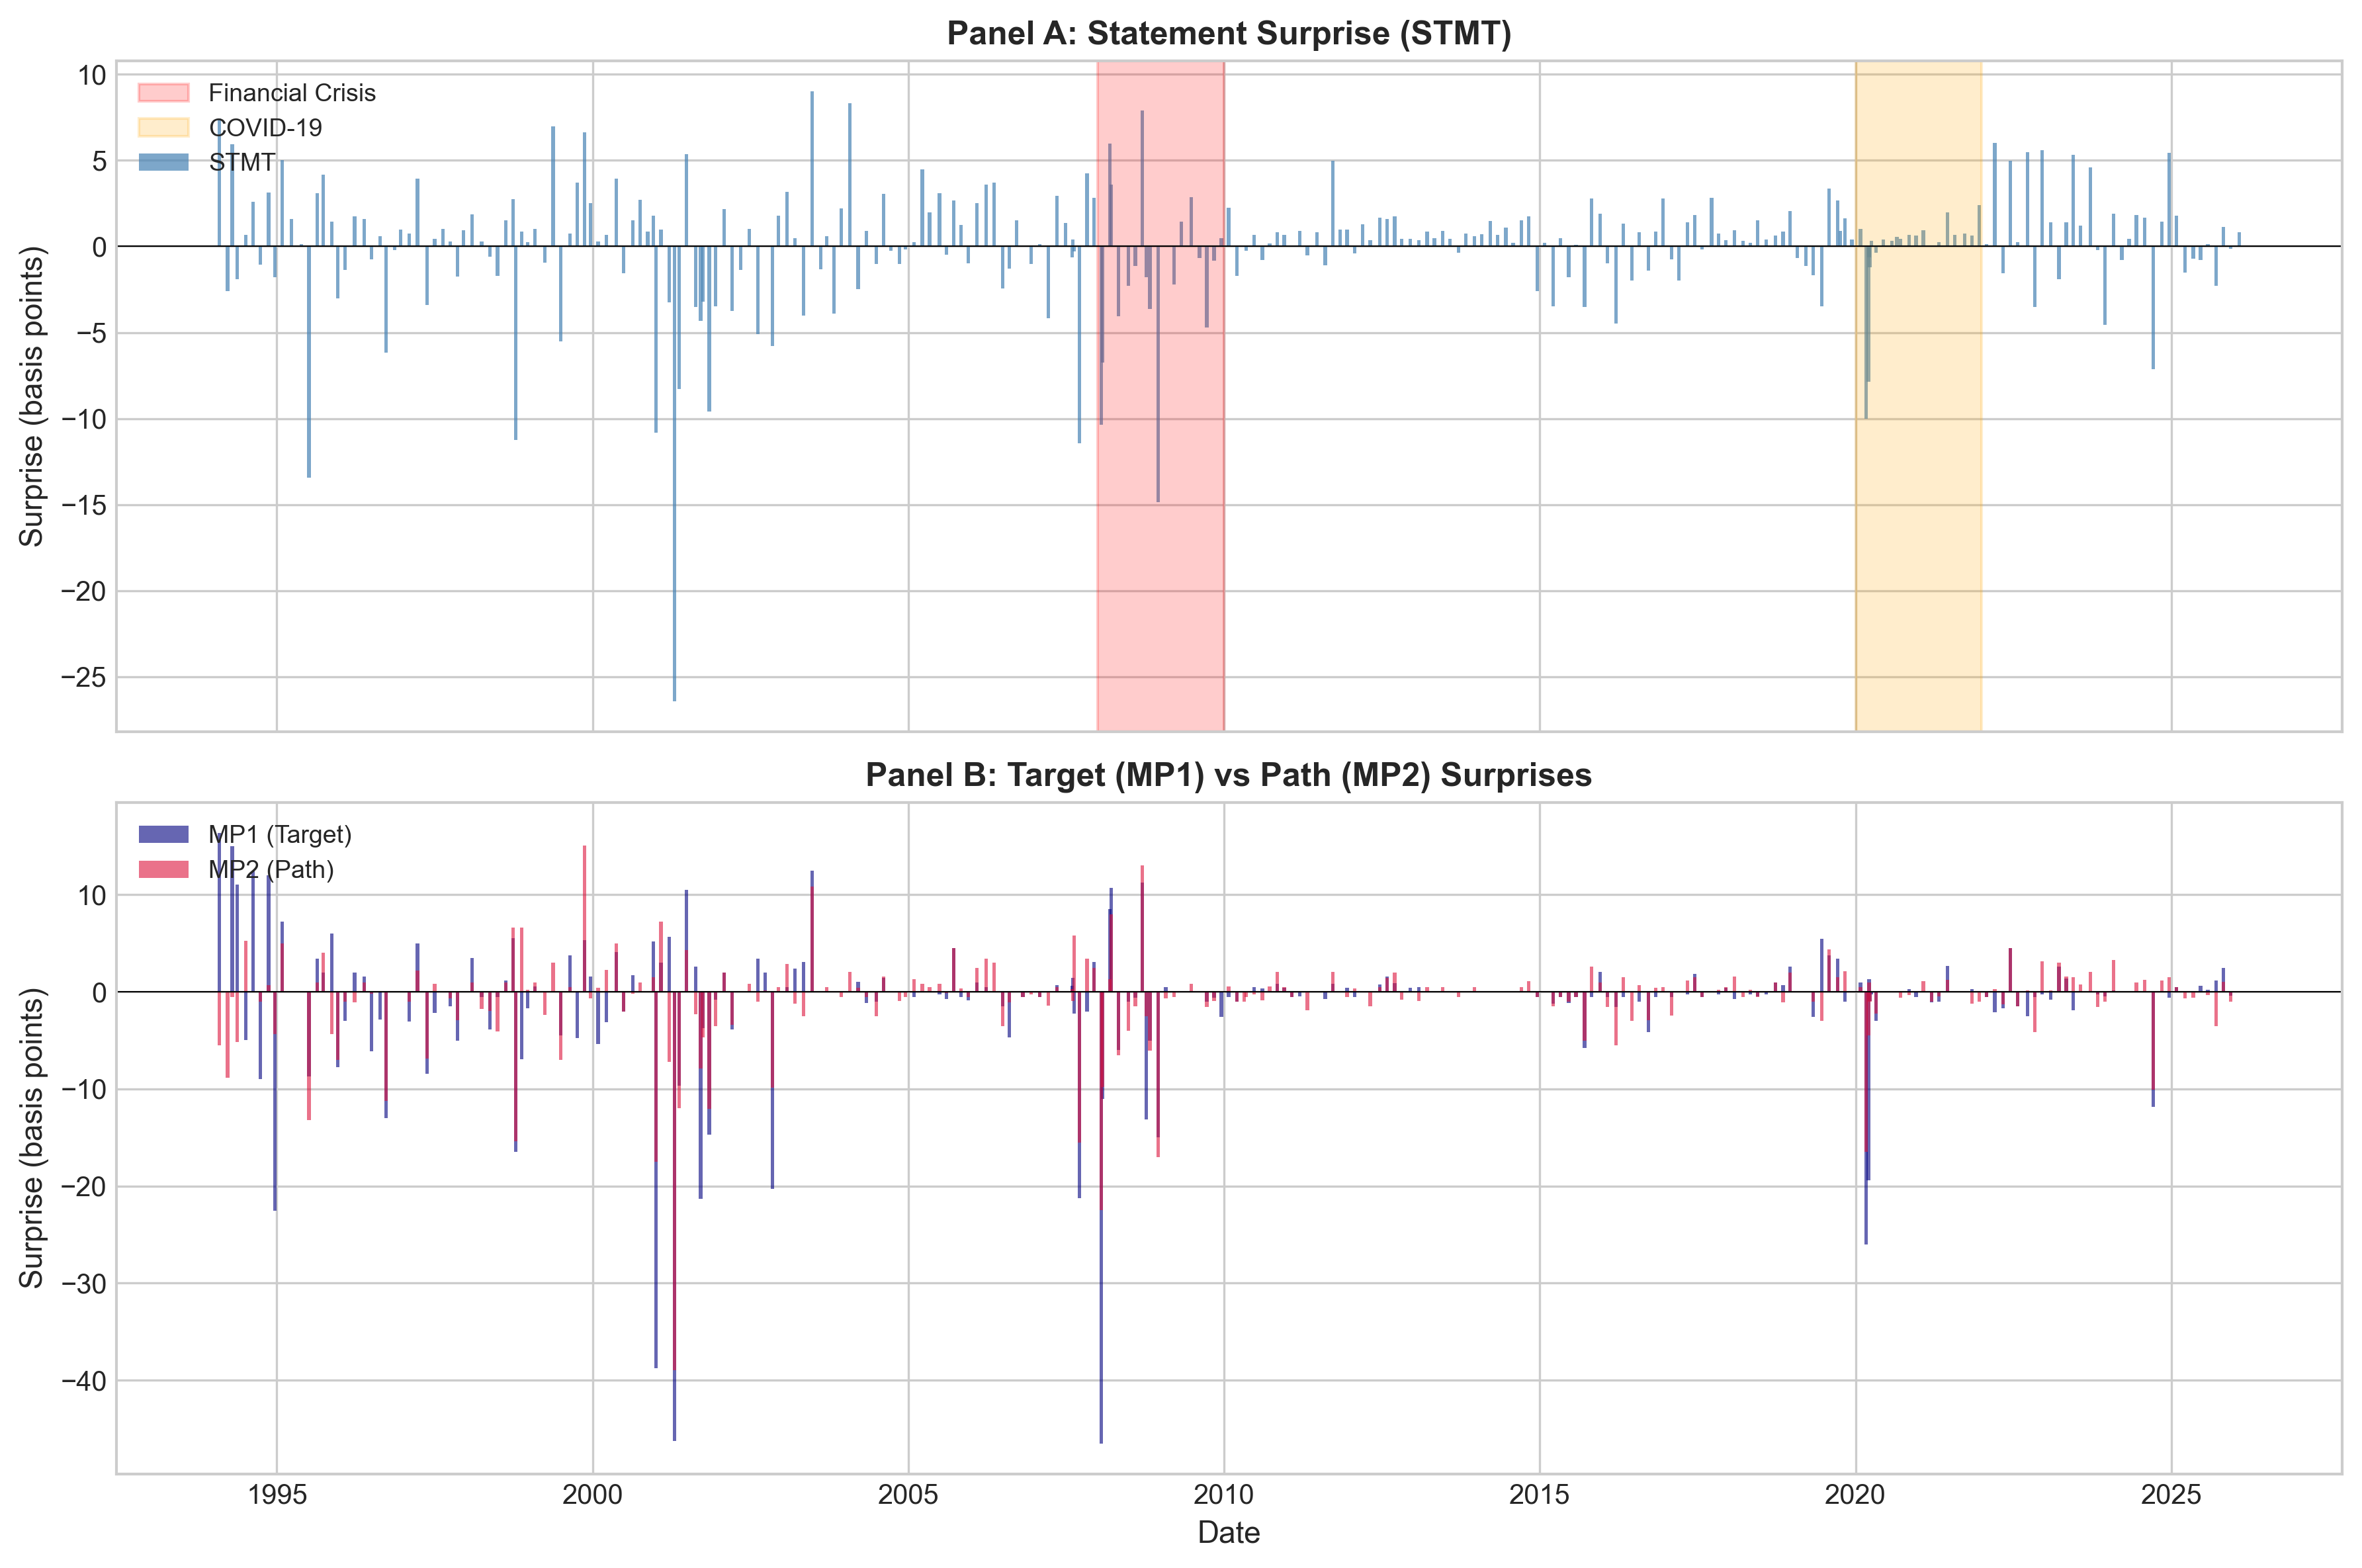
\includegraphics[width=0.9\textwidth]{figure1_surprise_timeseries.png}
\caption{\textbf{Monetary Policy Surprises Over Time.} The STMT series shows large negative surprises in crisis episodes (2008--2009, 2020) and positive surprises during 2022--2024 tightening. This time variation motivates regime-split tests.}
\label{fig:surprise_timeseries}
\end{figure}

\begin{figure}
\centering
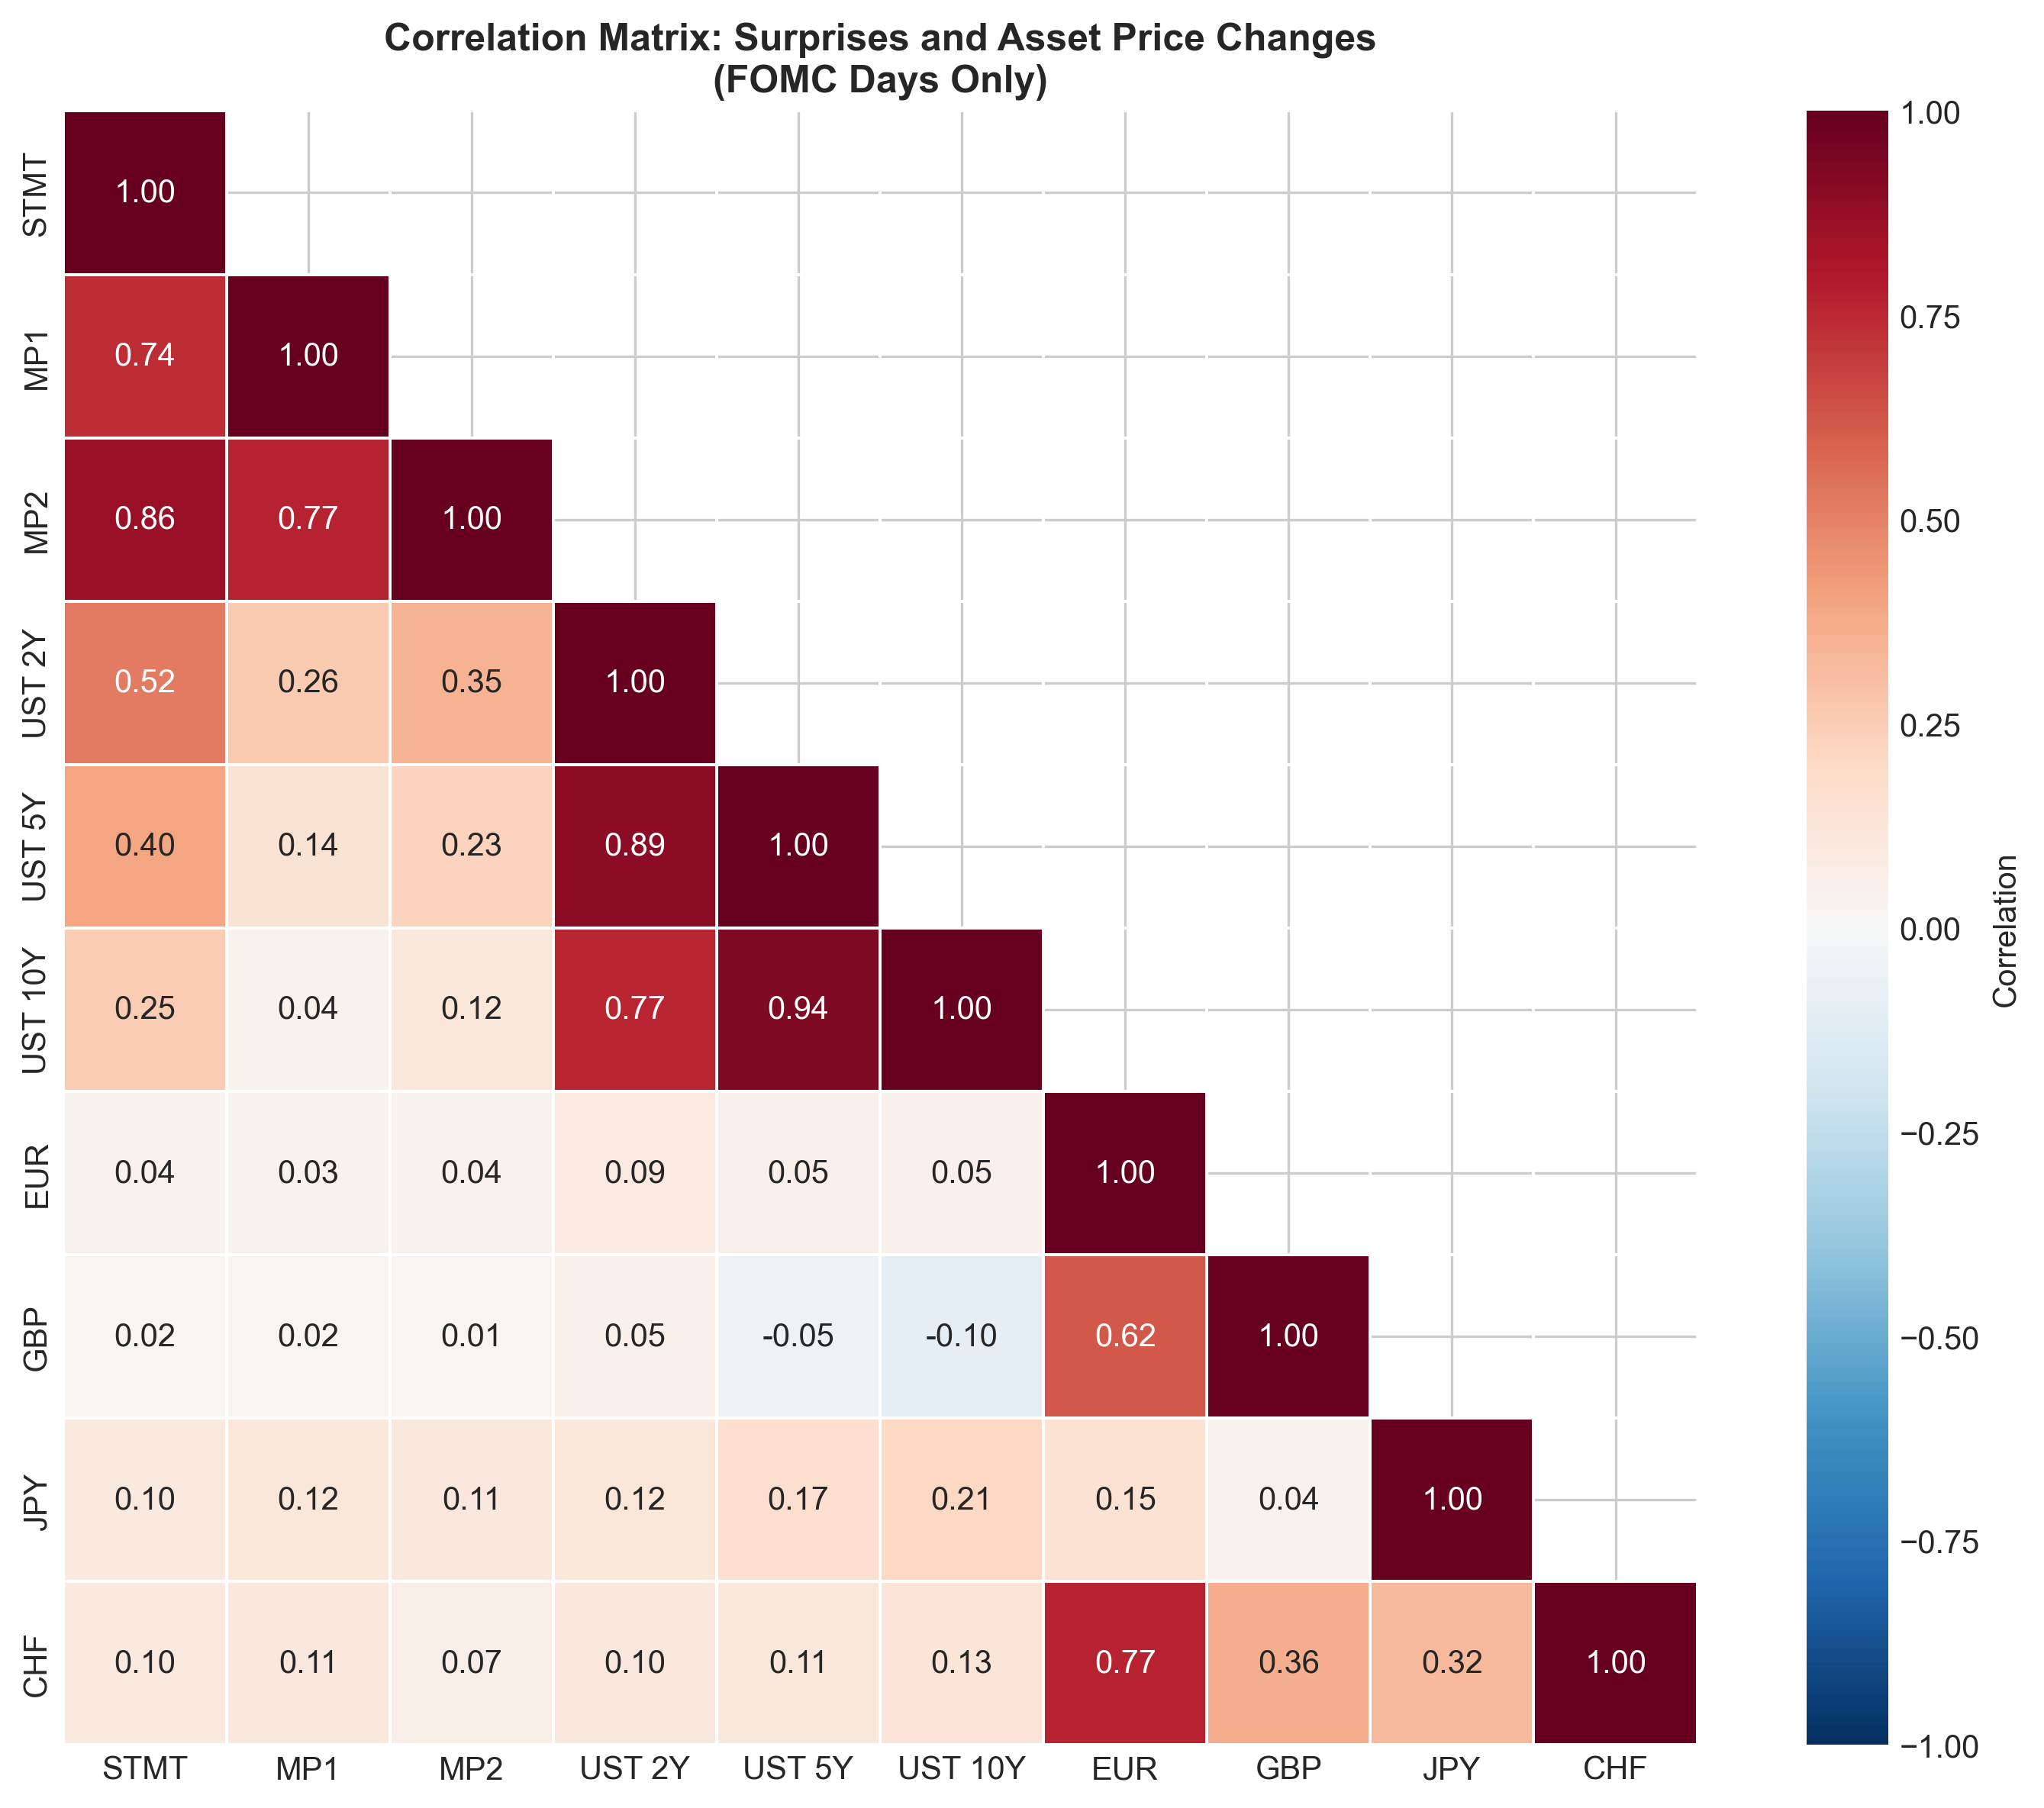
\includegraphics[width=0.85\textwidth]{figure2_correlation_heatmap.png}
\caption{\textbf{Correlation Among Surprise Measures.} STMT correlates highly with both MP1 and MP2, indicating it loads on multiple dimensions of monetary news.}
\label{fig:surprise_correlation}
\end{figure}

\begin{figure}
\centering
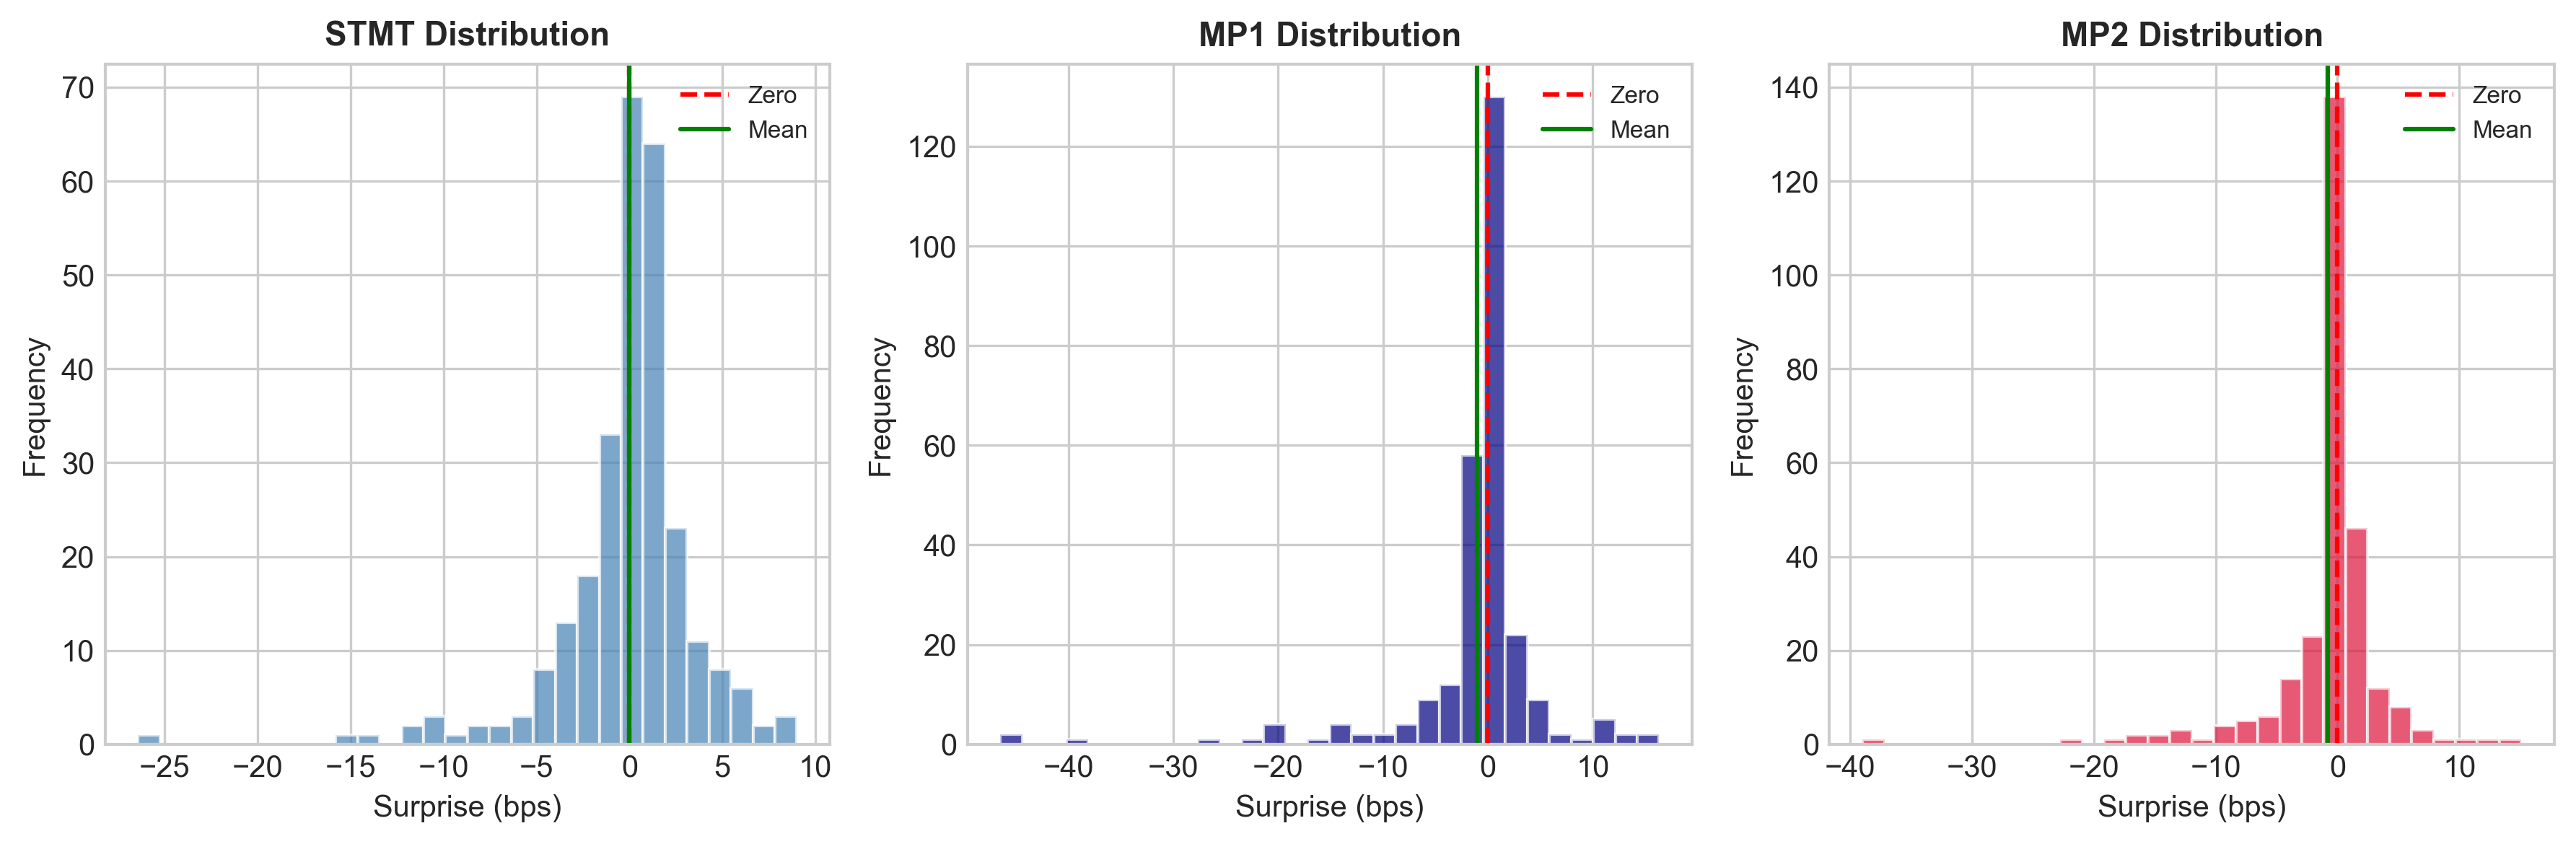
\includegraphics[width=0.85\textwidth]{figure3_surprise_distributions.png}
\caption{\textbf{Distribution of Surprise Measures.} Means near zero (market efficiency) with fat tails (rare large shocks). Outliers from crisis announcements contribute disproportionately to identification.}
\label{fig:surprise_distribution}
\end{figure}

\begin{figure}
\centering
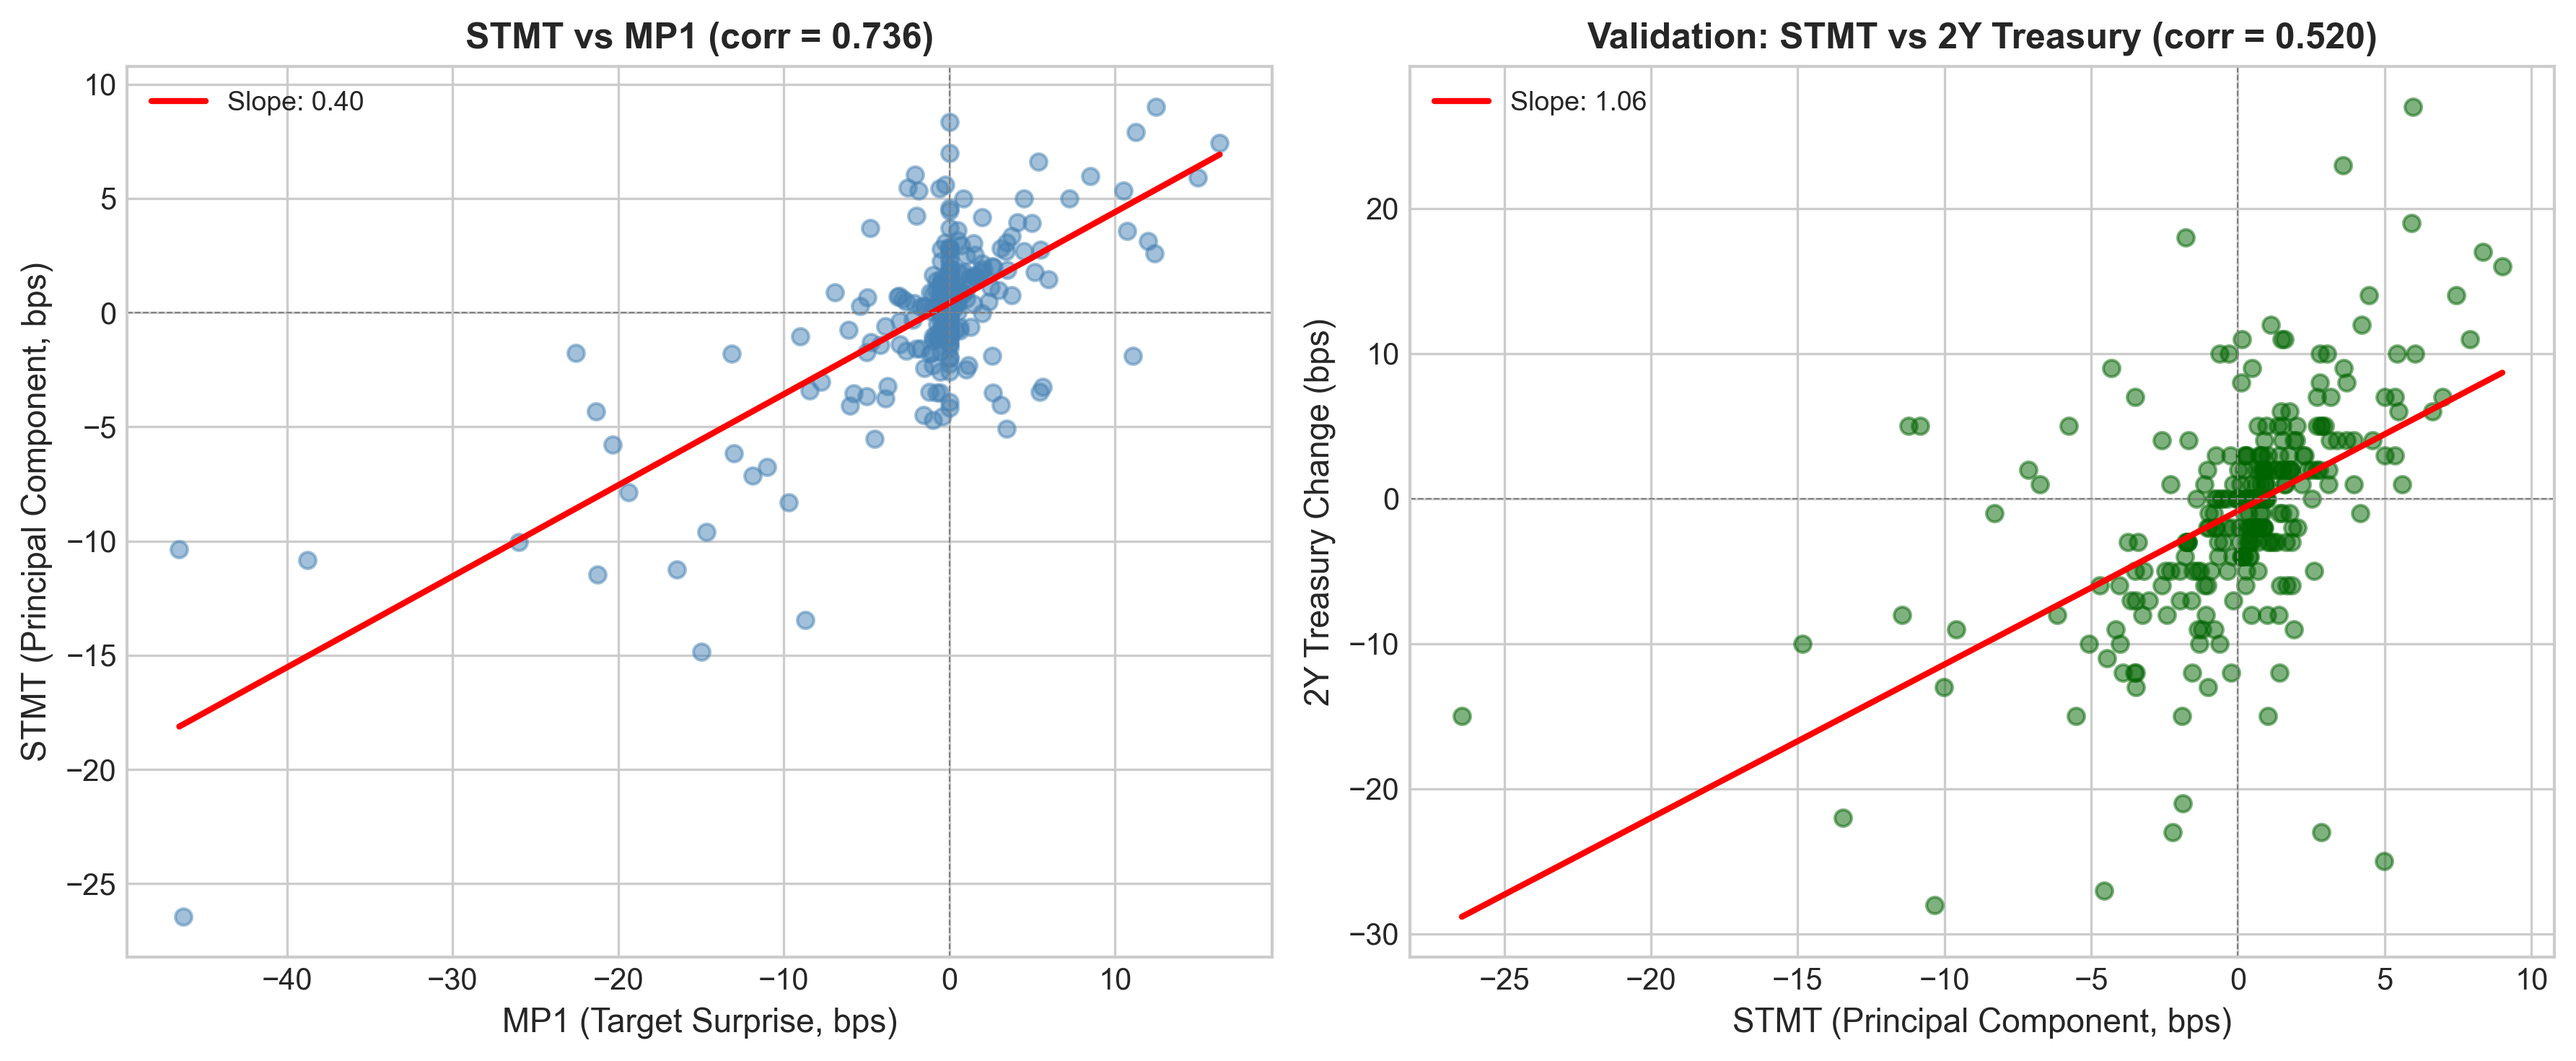
\includegraphics[width=0.9\textwidth]{figure4_stmt_validation.png}
\caption{\textbf{External Validation: STMT vs Treasury Yield Changes.} Tight positive relationship confirms STMT captures policy-relevant news that moves the yield curve.}
\label{fig:stmt_validation}
\end{figure}

\begin{figure}
\centering
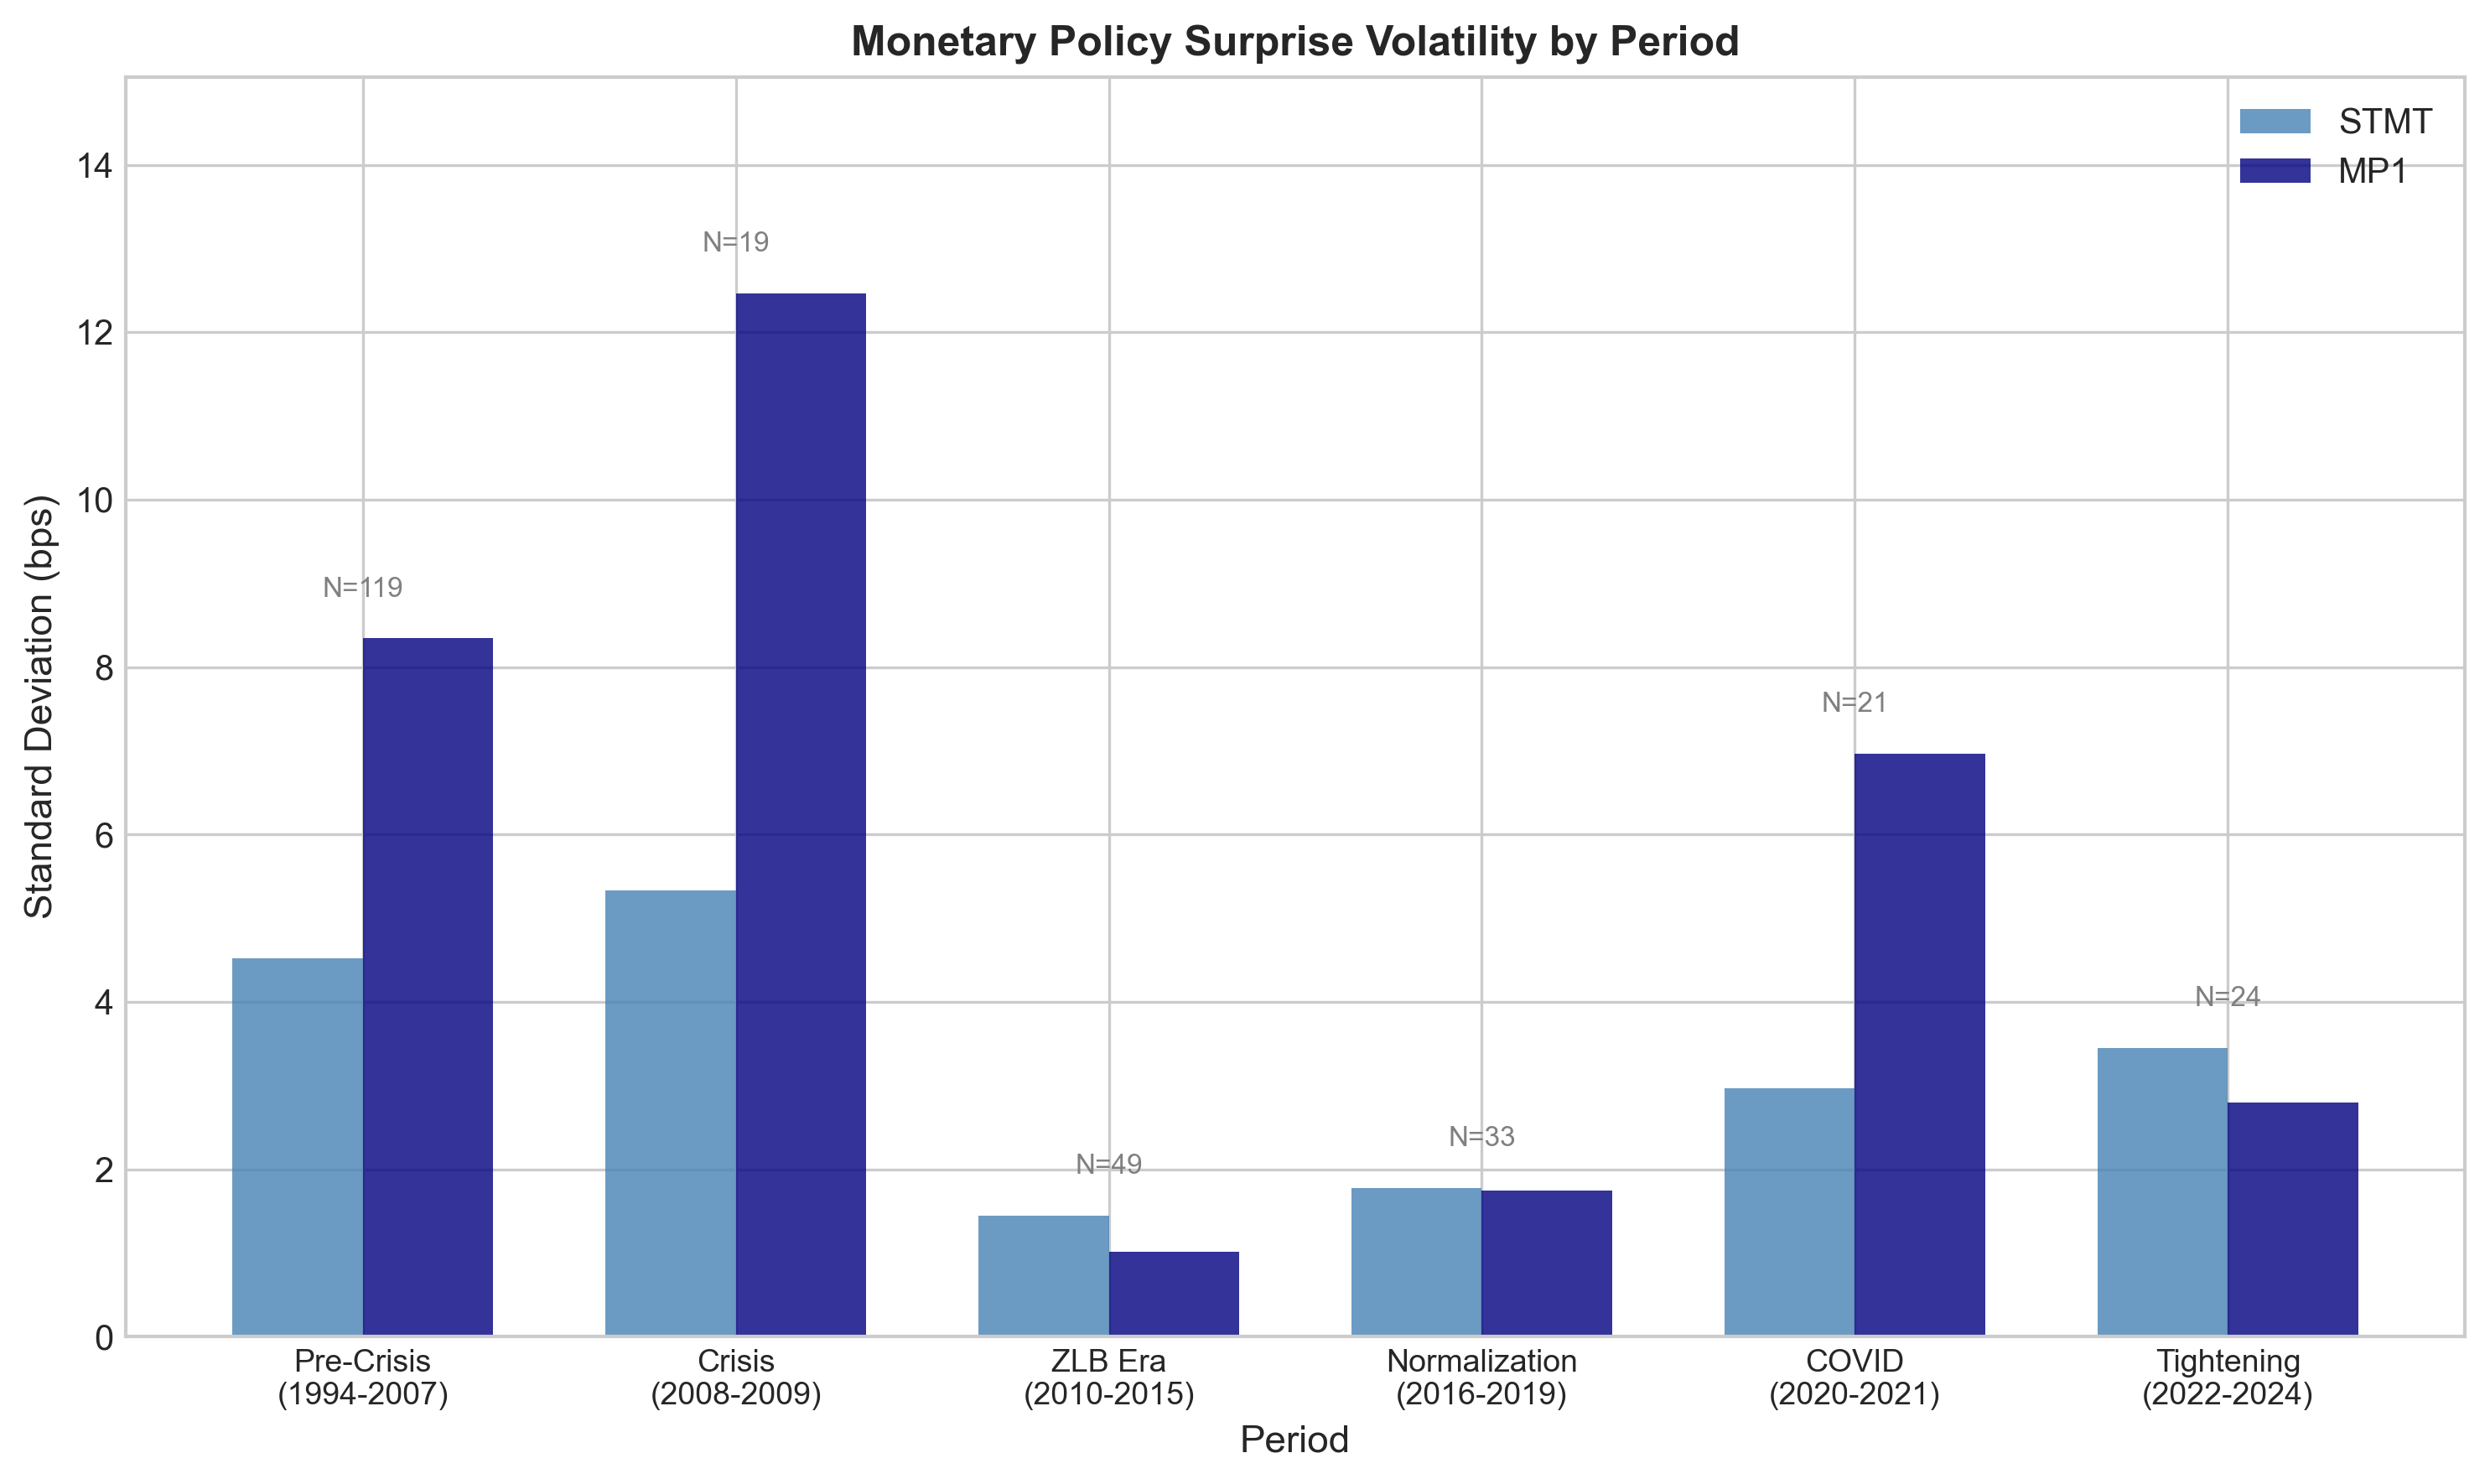
\includegraphics[width=0.85\textwidth]{figure6_volatility_by_period.png}
\caption{\textbf{Surprise Volatility by Monetary Regime.} Volatility is higher in crisis periods, motivating regime-interaction specifications.}
\label{fig:volatility_regimes}
\end{figure}

\begin{figure}
\centering
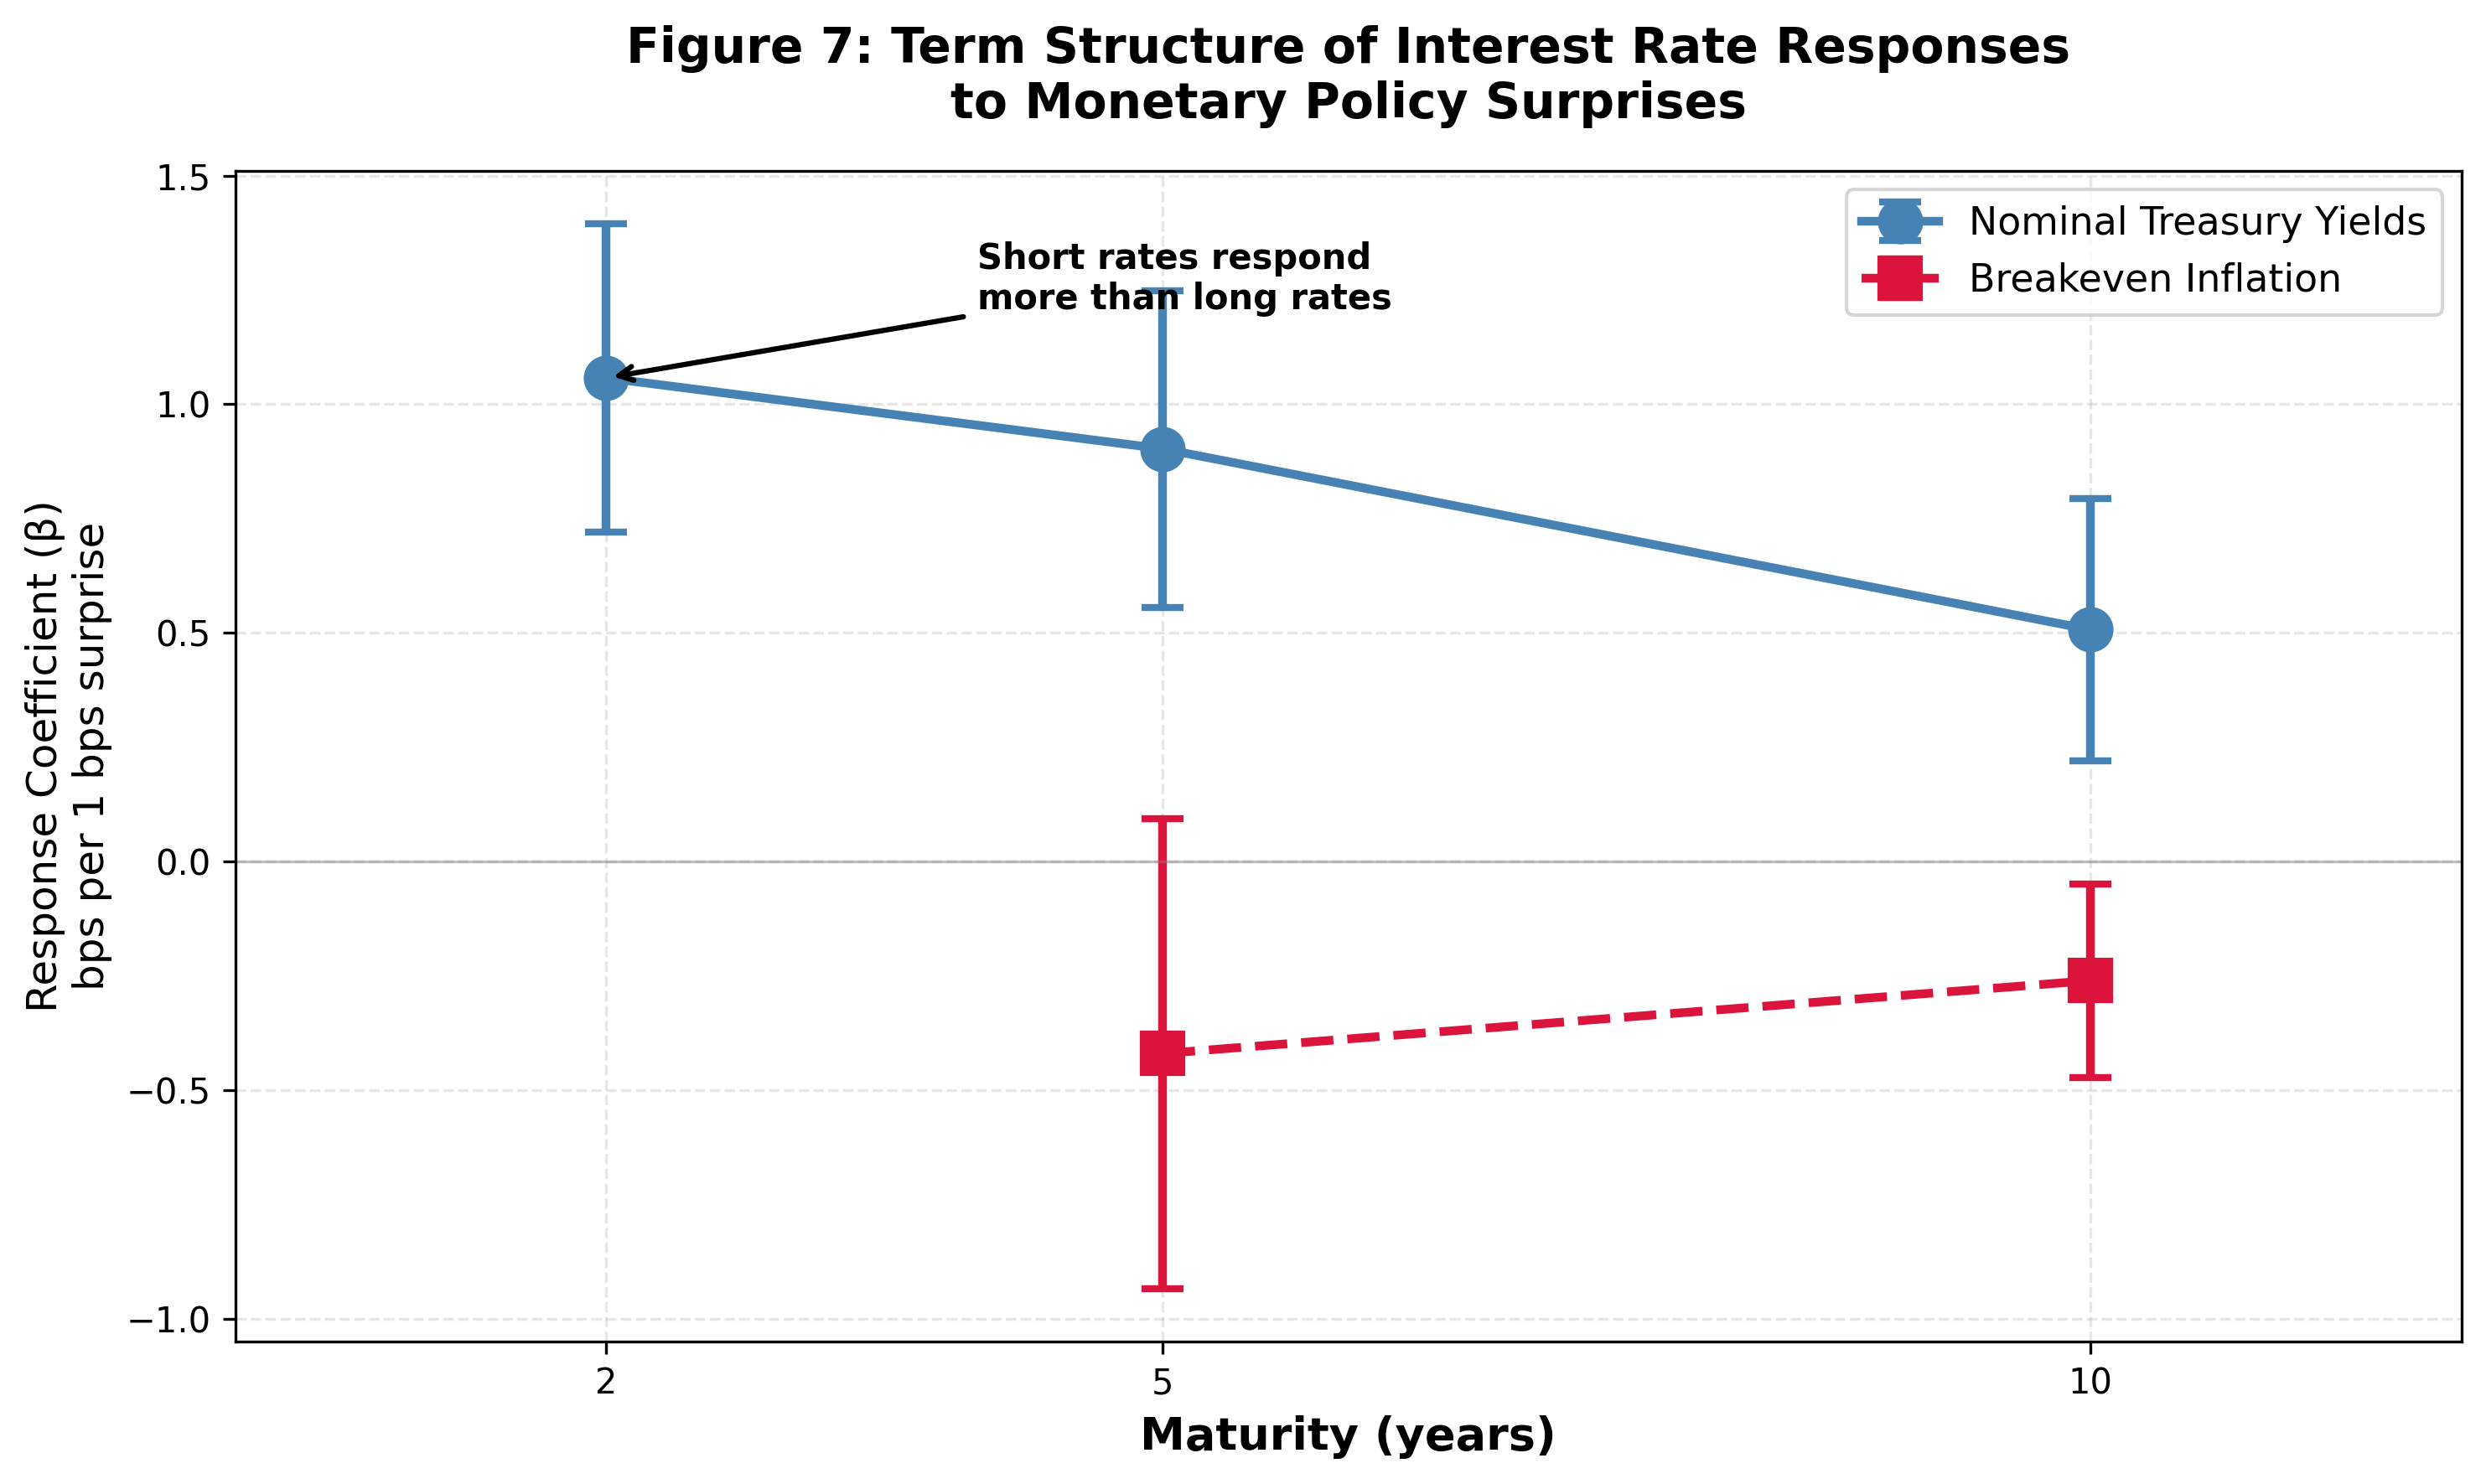
\includegraphics[width=0.85\textwidth]{figure7_term_structure.png}
\caption{\textbf{Treasury Yield Coefficients by Maturity.} Declining response with maturity: short rates respond most, consistent with conventional monetary transmission.}
\label{fig:treasury_coefficients}
\end{figure}

\begin{figure}
\centering
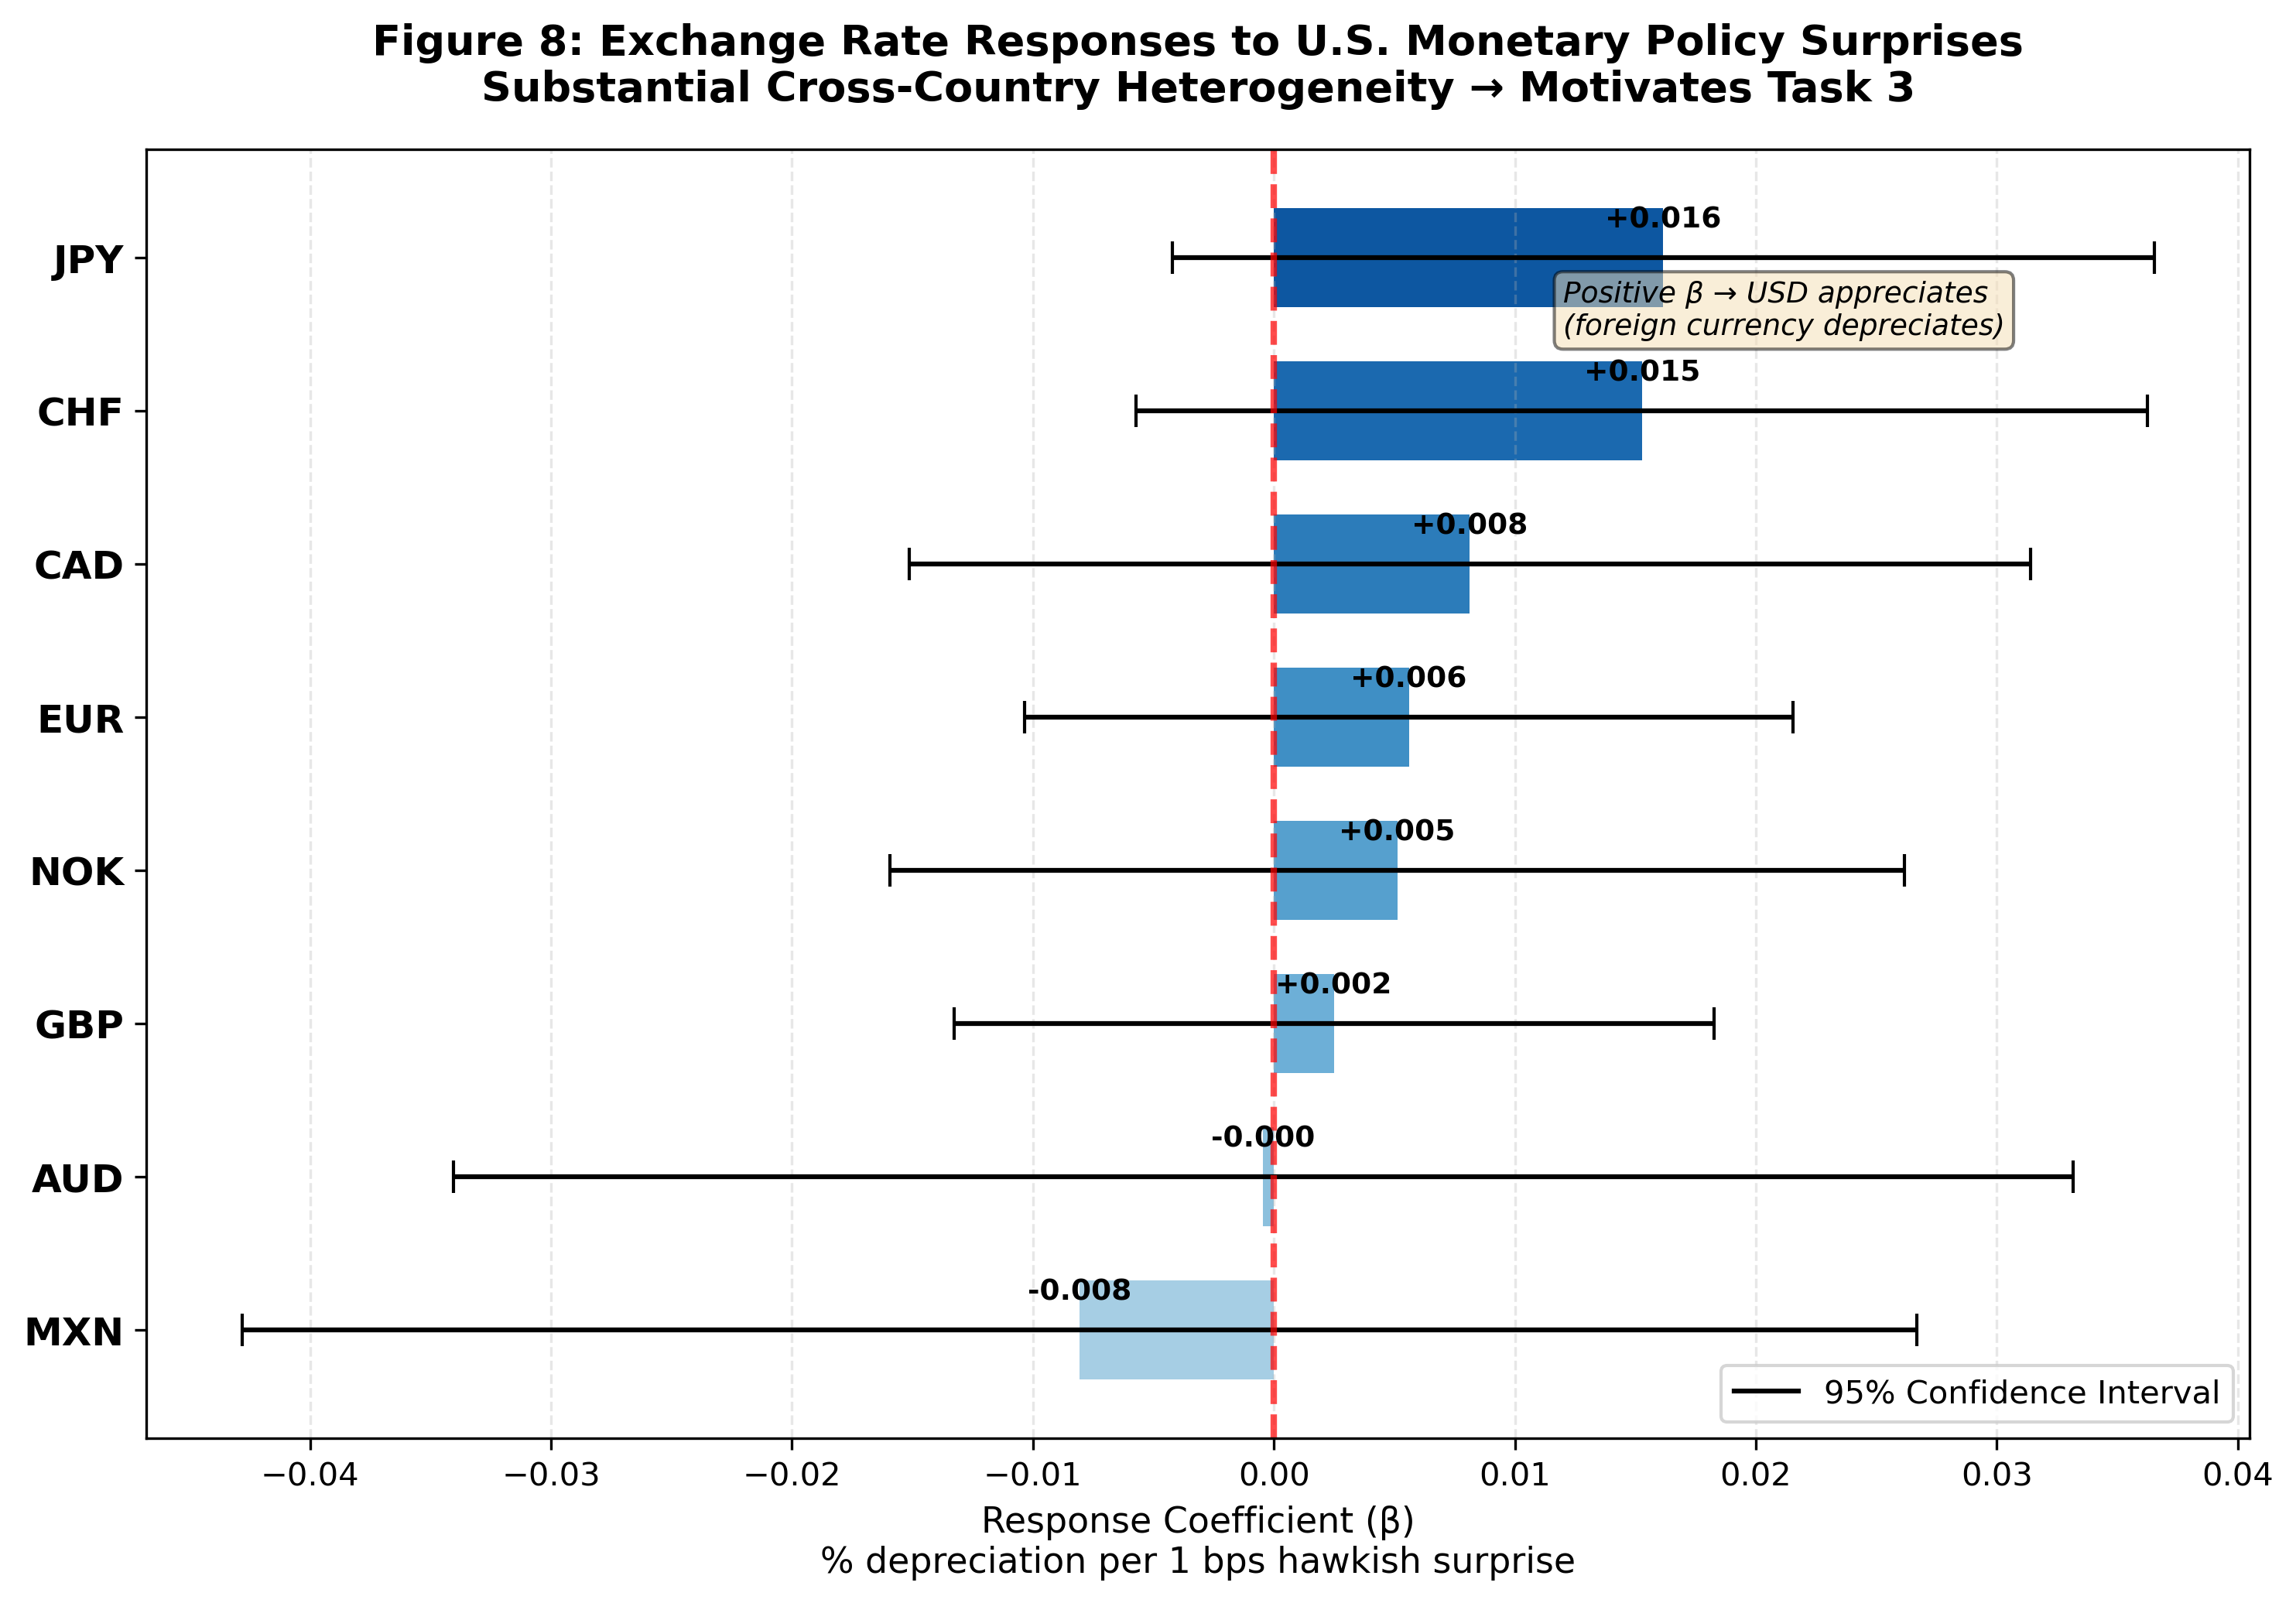
\includegraphics[width=0.85\textwidth]{figure8_fx_heterogeneity.png}
\caption{\textbf{Exchange Rate Coefficients by Currency.} All negative (hawkish $\rightarrow$ foreign depreciation) but imprecisely estimated. Cross-currency dispersion motivates mechanism test.}
\label{fig:fx_coefficients}
\end{figure}

\begin{figure}
\centering
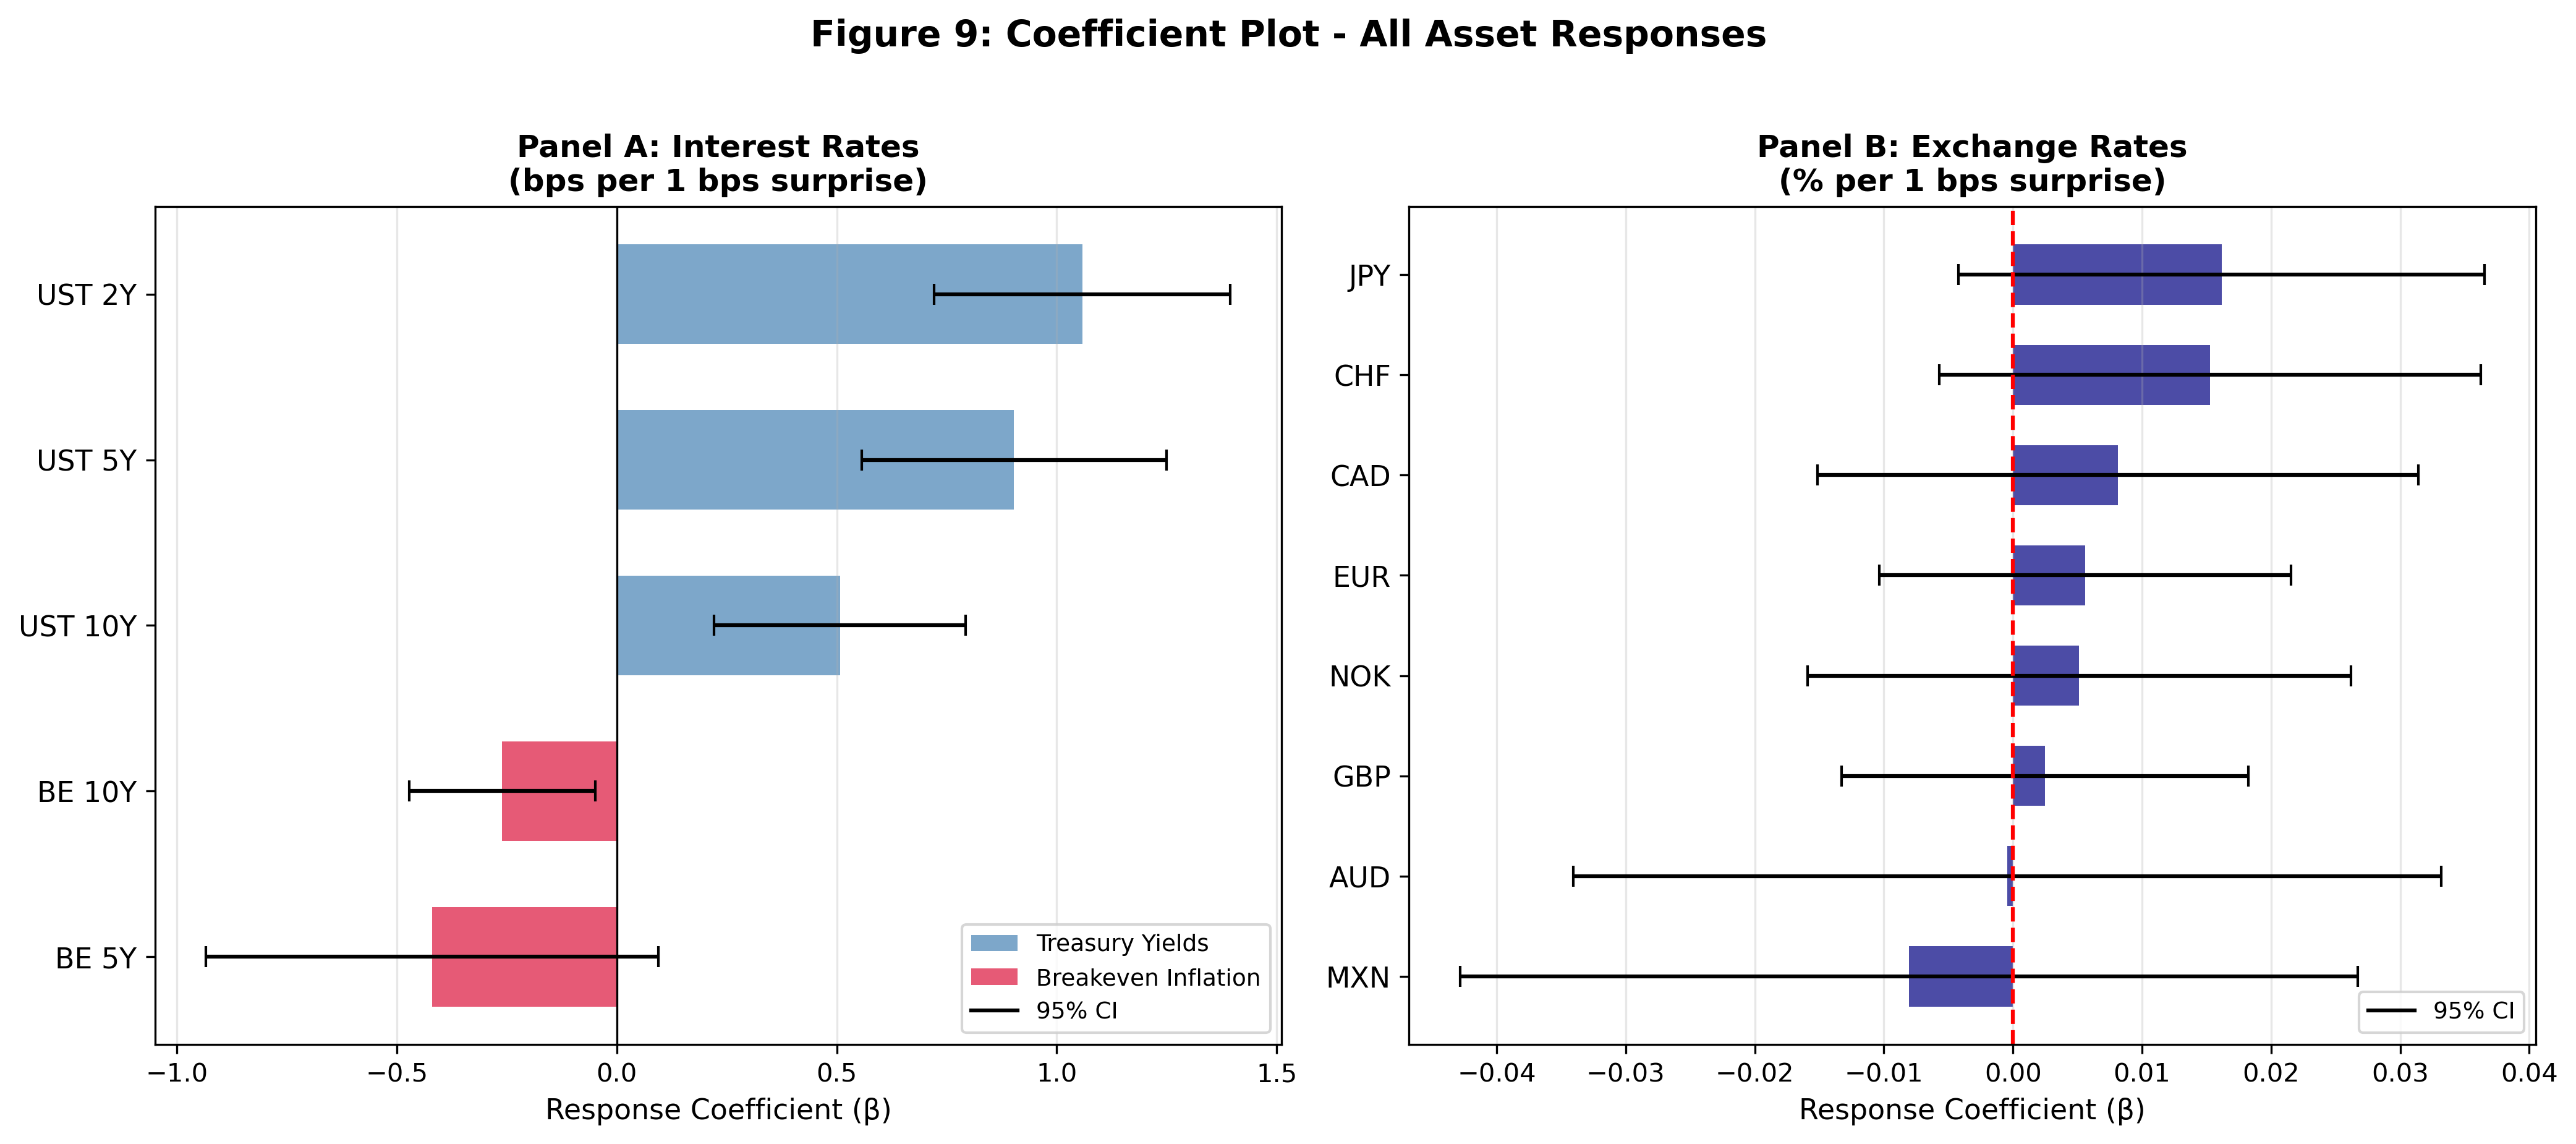
\includegraphics[width=0.9\textwidth]{figure9_coefficient_plot.png}
\caption{\textbf{Yields vs FX: Response Comparison.} Treasury yields respond sharply and precisely; FX responses are small relative to daily volatility.}
\label{fig:unified_coefficients}
\end{figure}

\begin{figure}
\centering
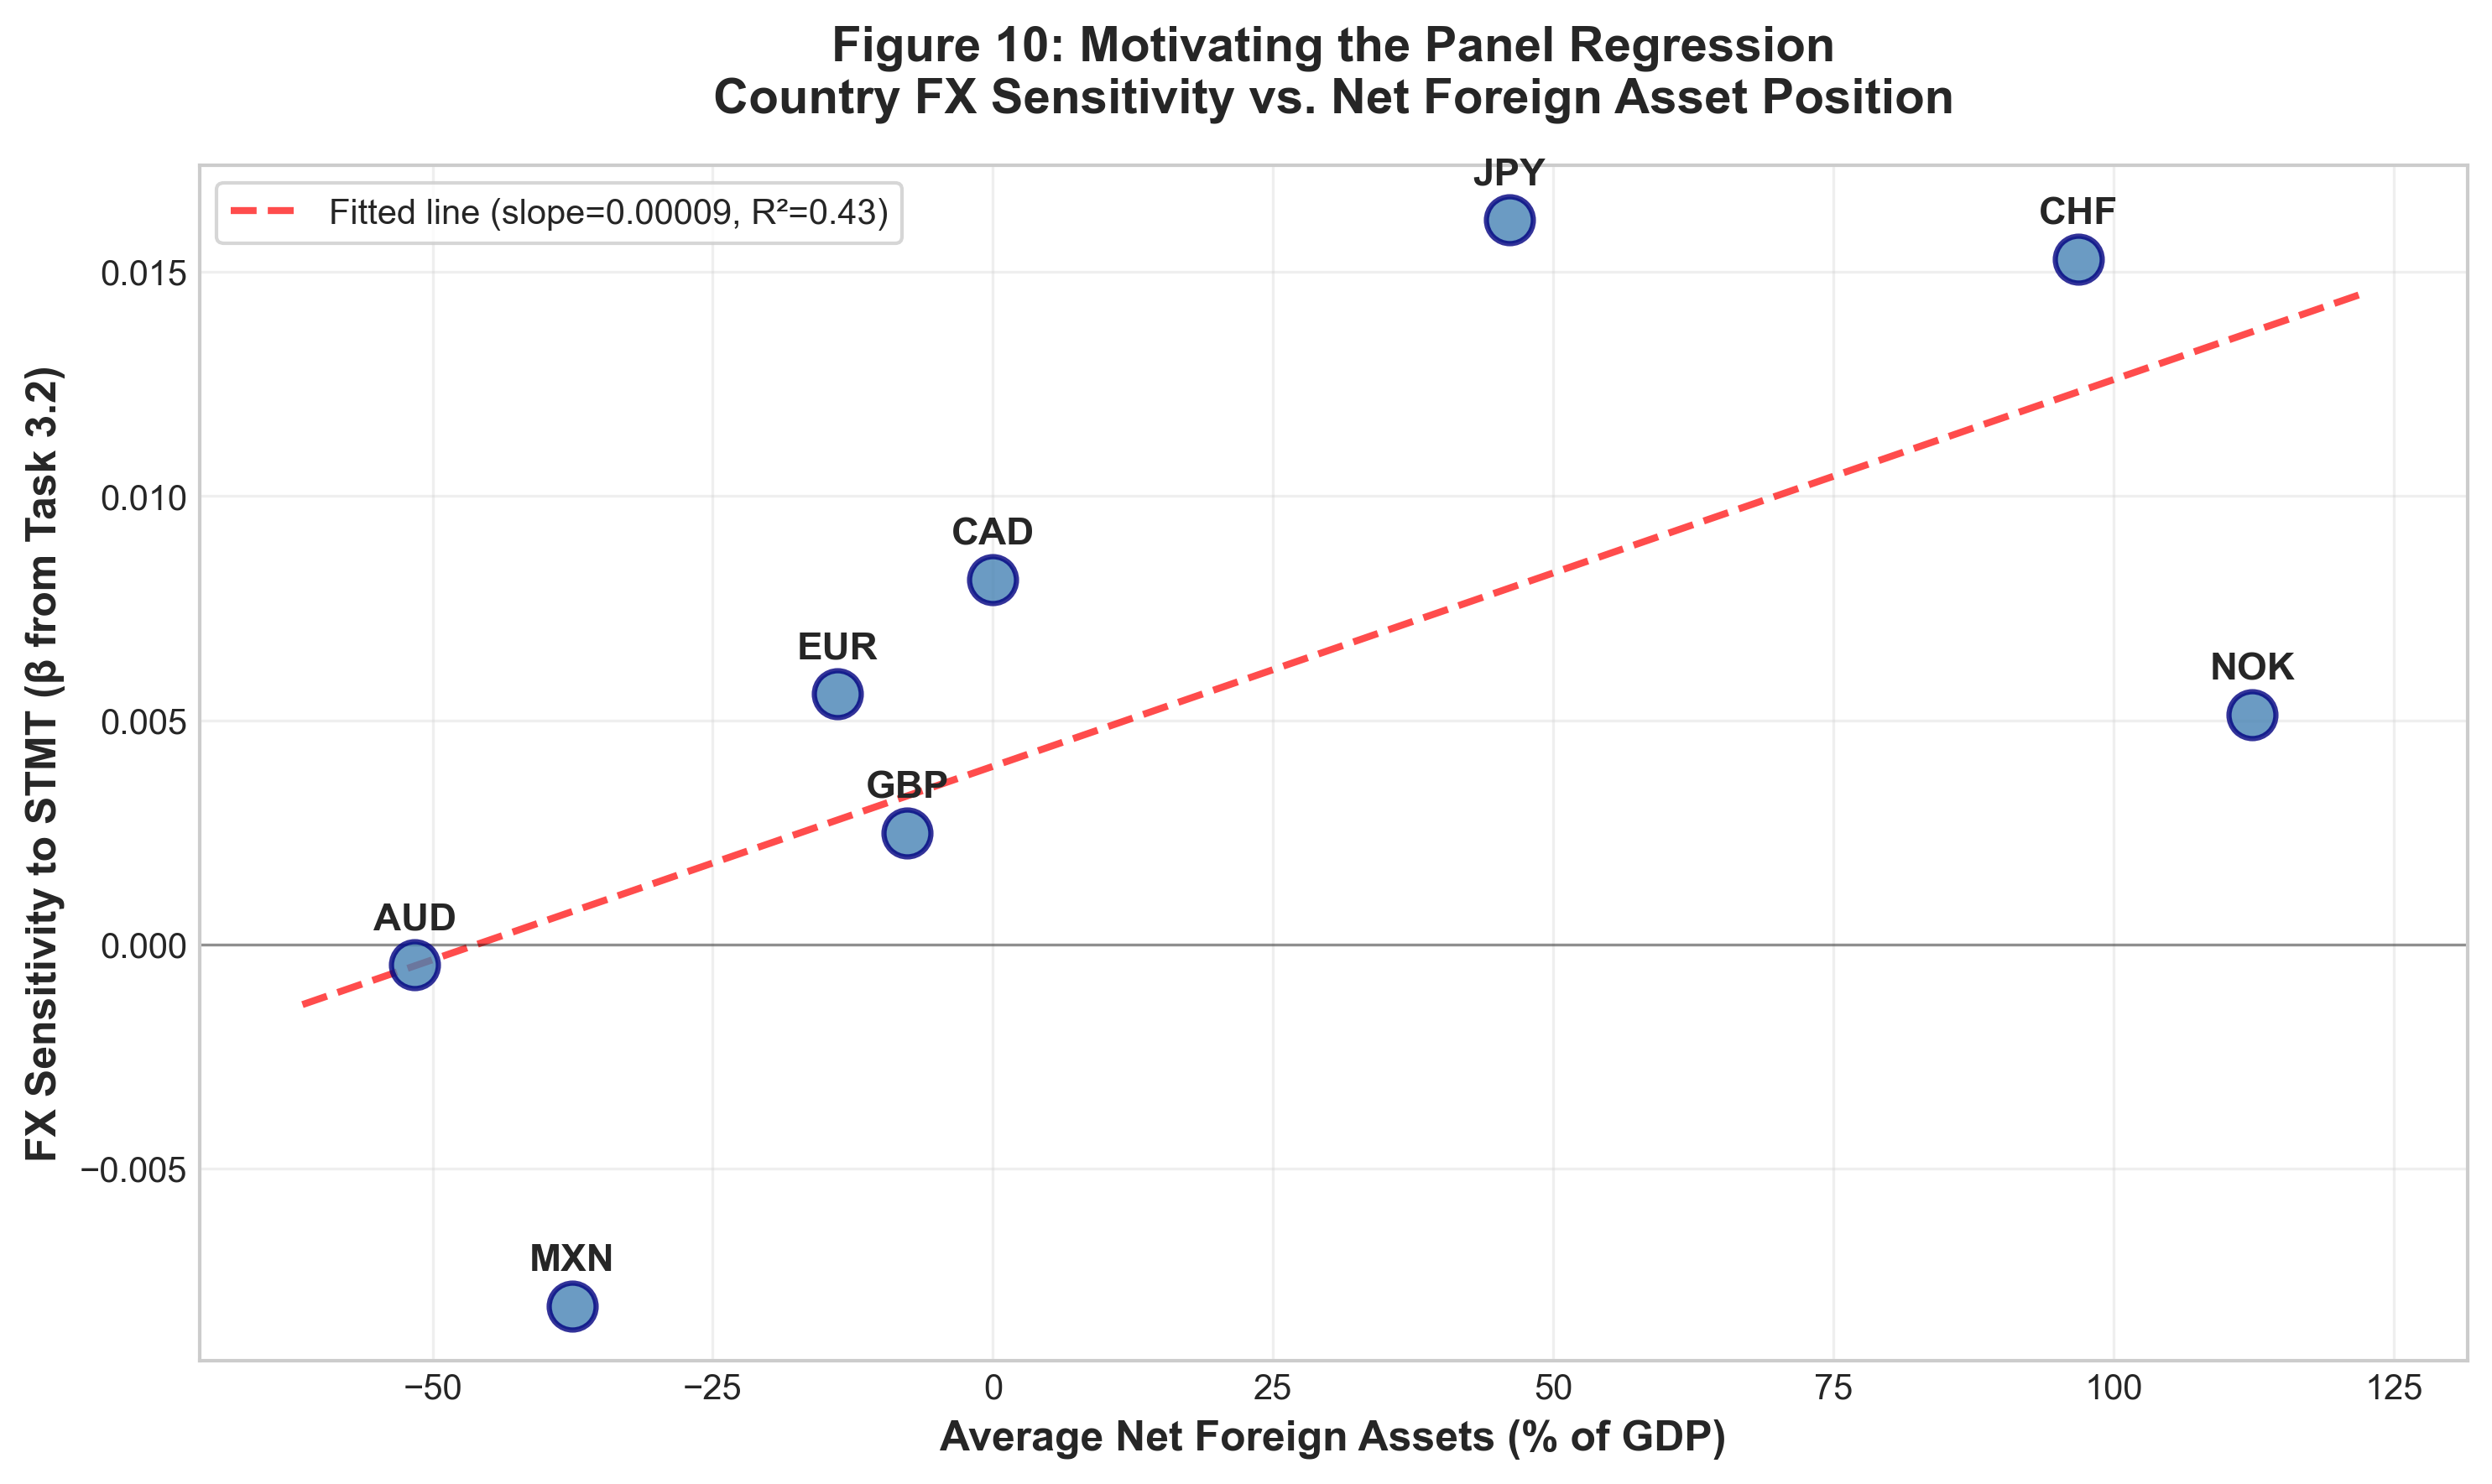
\includegraphics[width=0.85\textwidth]{figure10_betas_vs_nfa.png}
\caption{\textbf{Cross-Sectional Evidence: FX Sensitivity vs NFA/GDP.} Weak relationship sensitive to individual currencies. With 8 currencies, cross-section is low-powered.}
\label{fig:cross_section}
\end{figure}

\begin{figure}
\centering
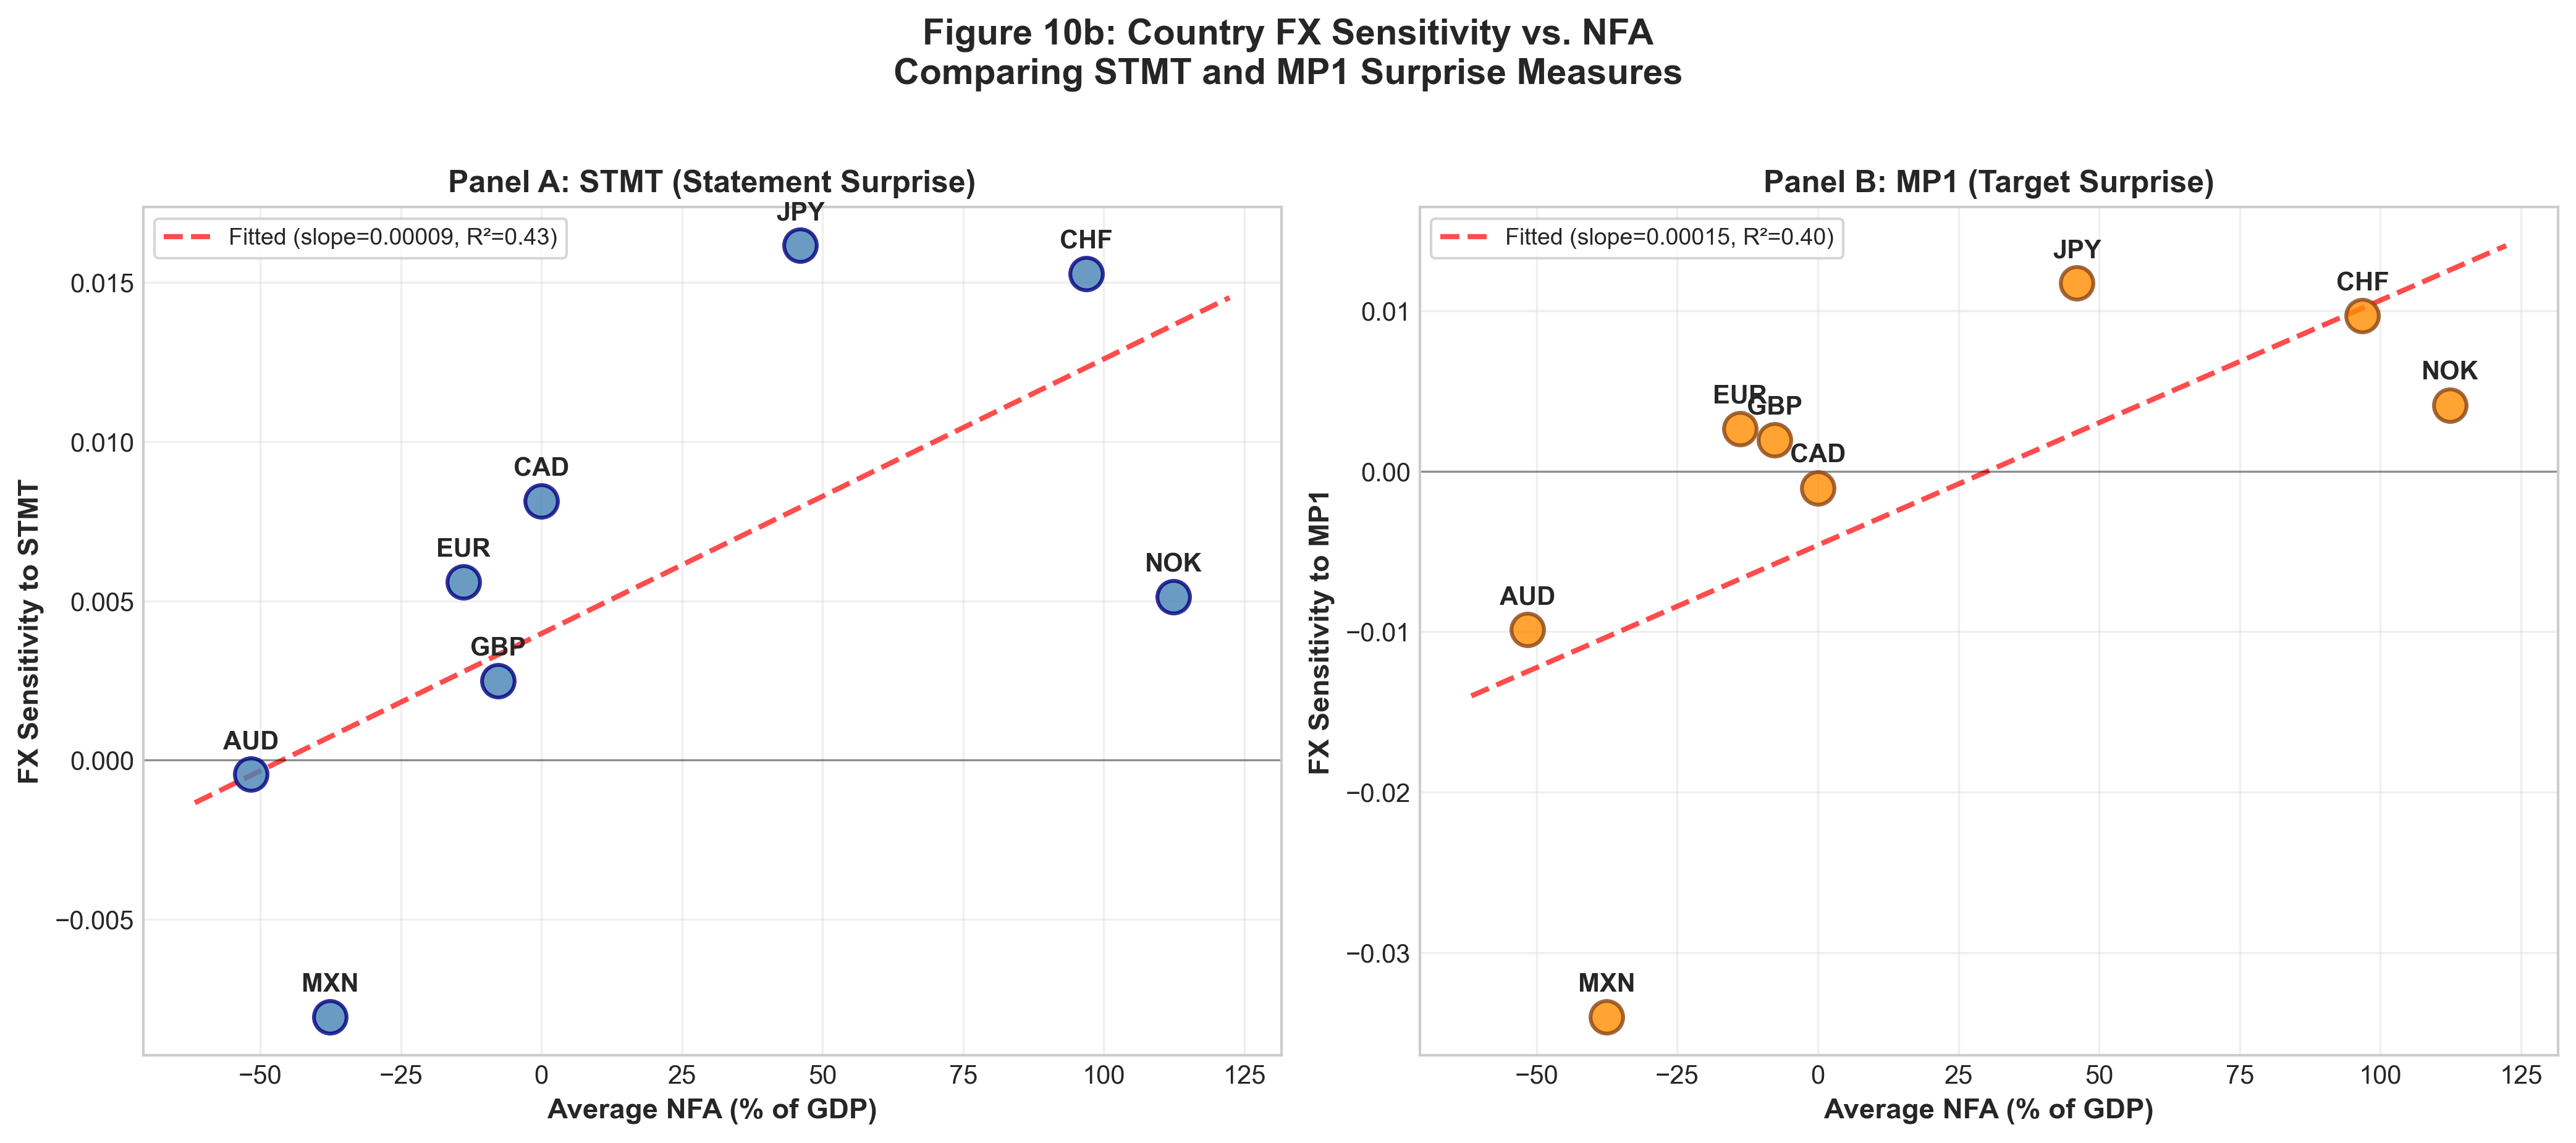
\includegraphics[width=0.85\textwidth]{figure10b_betas_vs_nfa_both.png}
\caption{\textbf{Cross-Section by Shock Definition.} Relationship differs across STMT vs MP1, suggesting any channel may depend on shock type.}
\label{fig:cross_section_by_shock}
\end{figure}

\begin{figure}
\centering
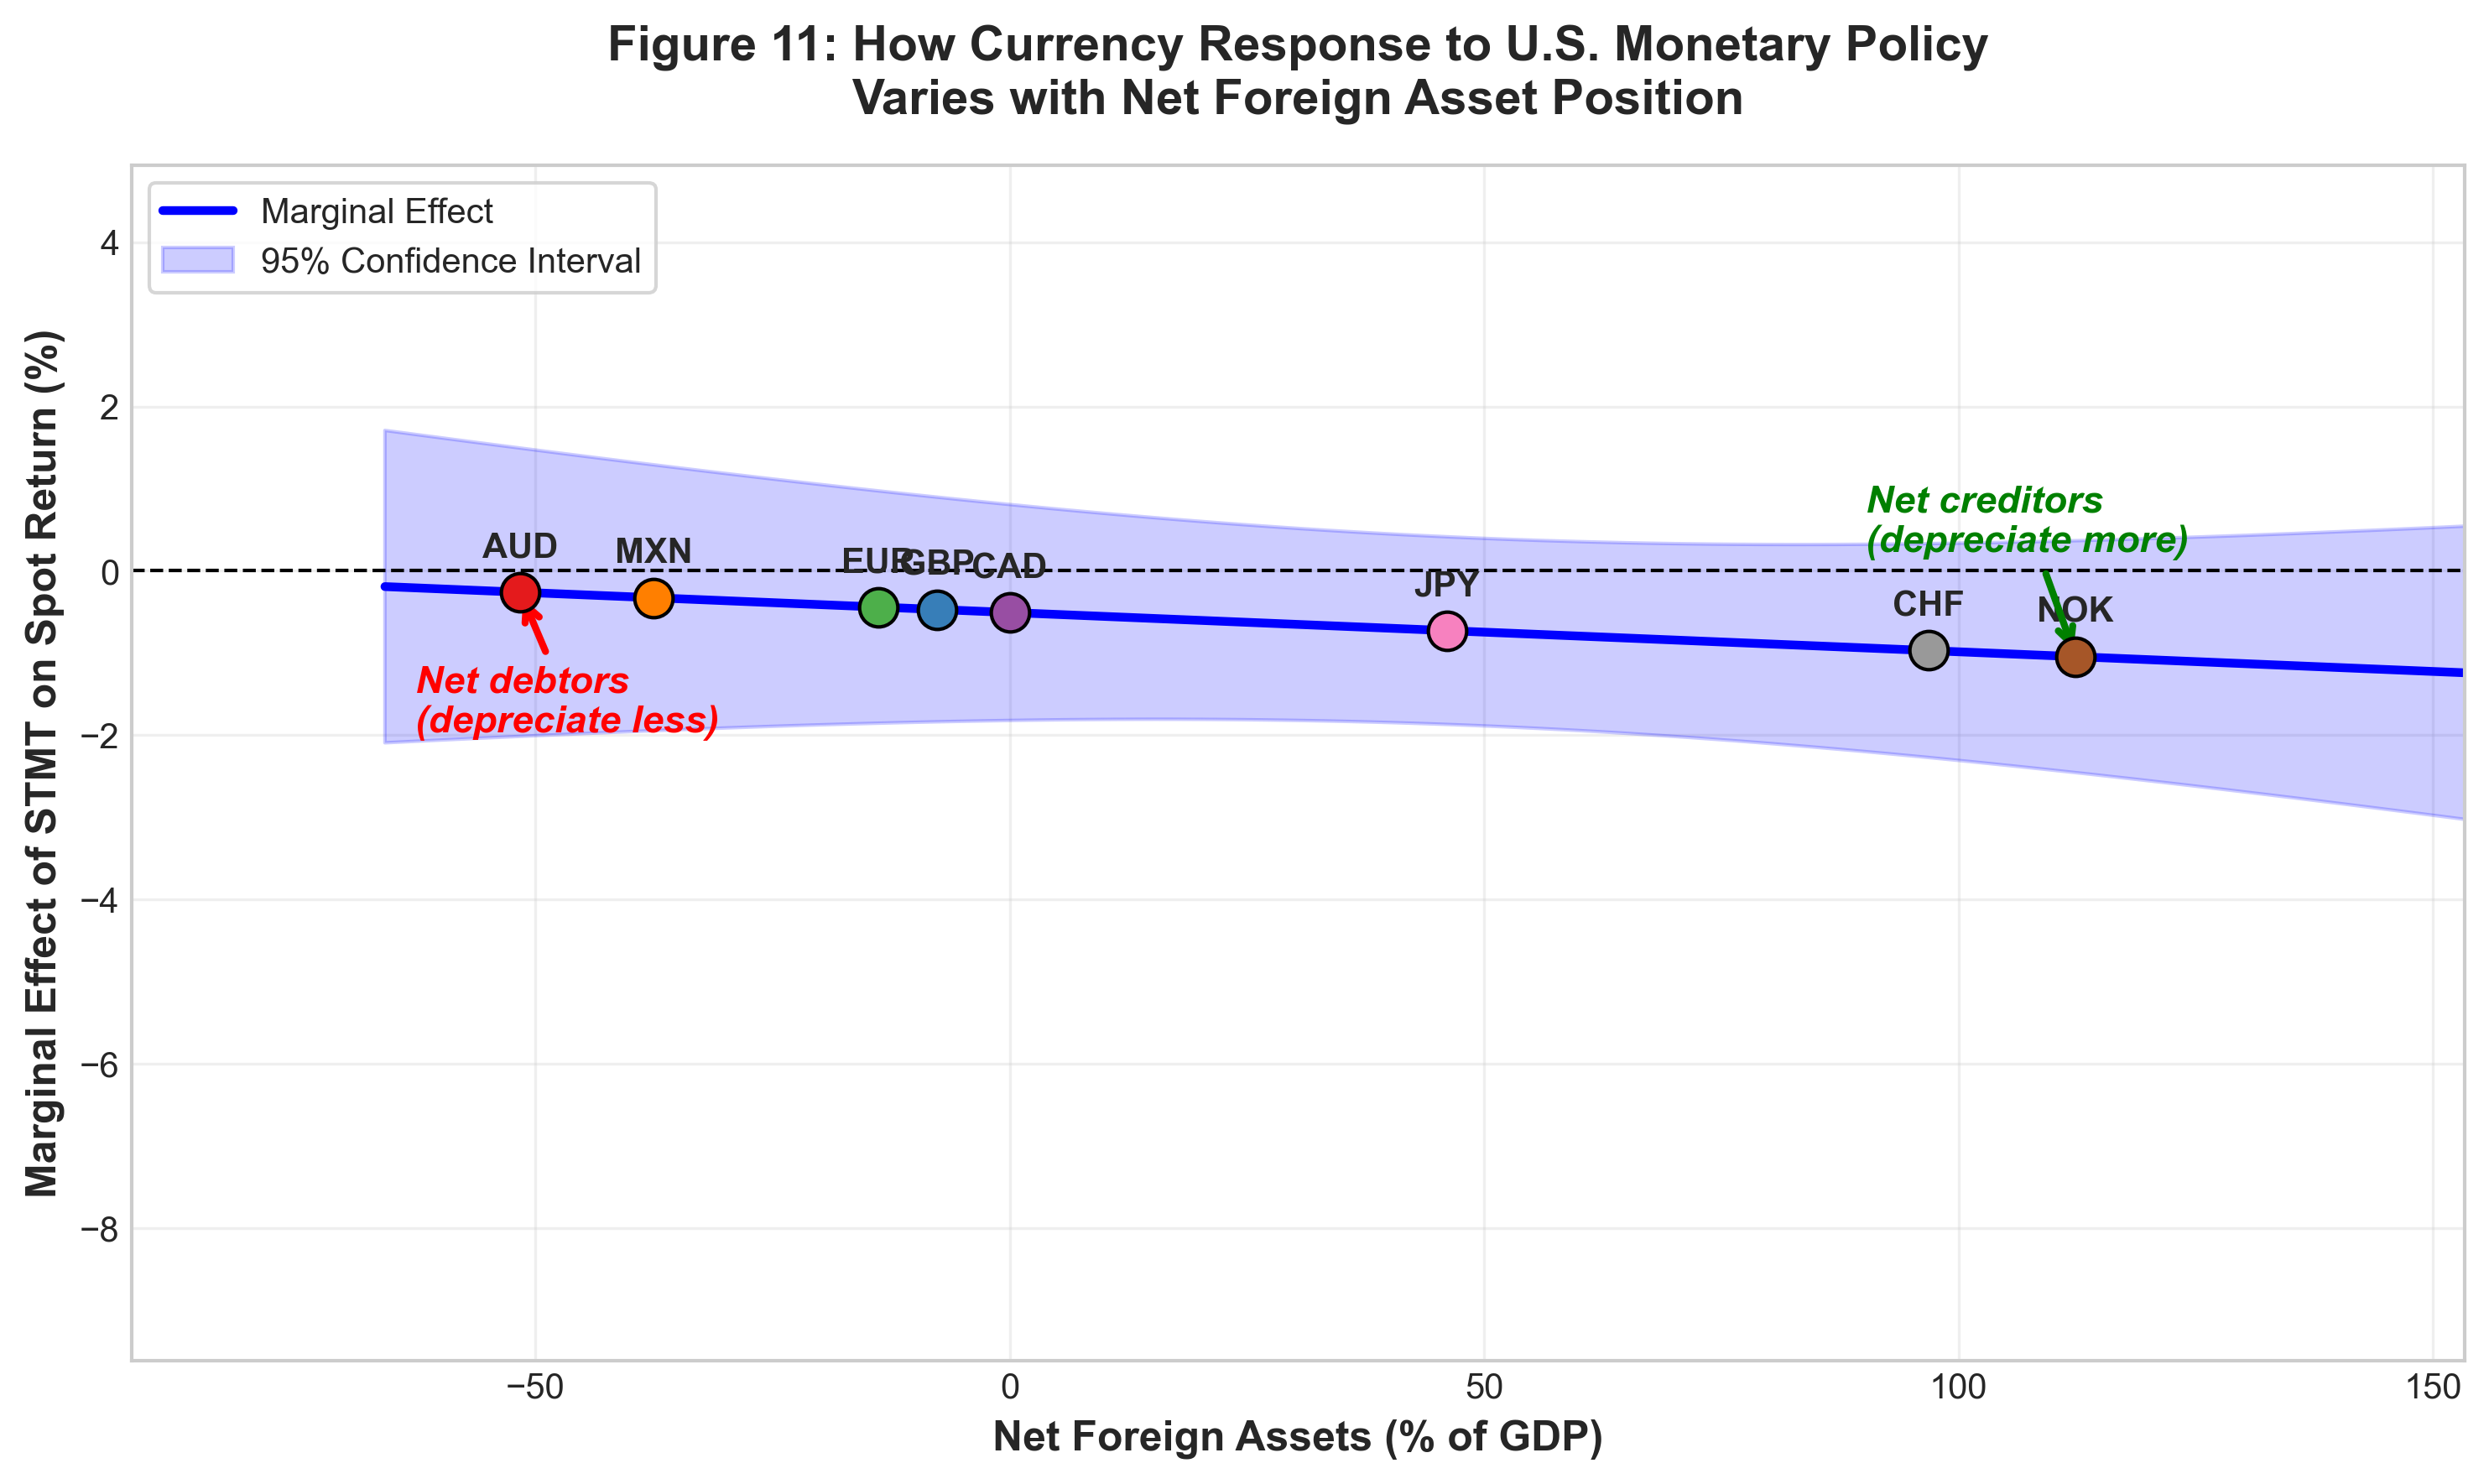
\includegraphics[width=0.9\textwidth]{figure11_marginal_effects.png}
\caption{\textbf{Marginal Effect of STMT Across NFA Distribution.} The mechanism object: $\partial r/\partial \text{STMT}$ as a function of NFA. Slope is small relative to confidence band.}
\label{fig:marginal_effects}
\end{figure}

\begin{figure}
\centering
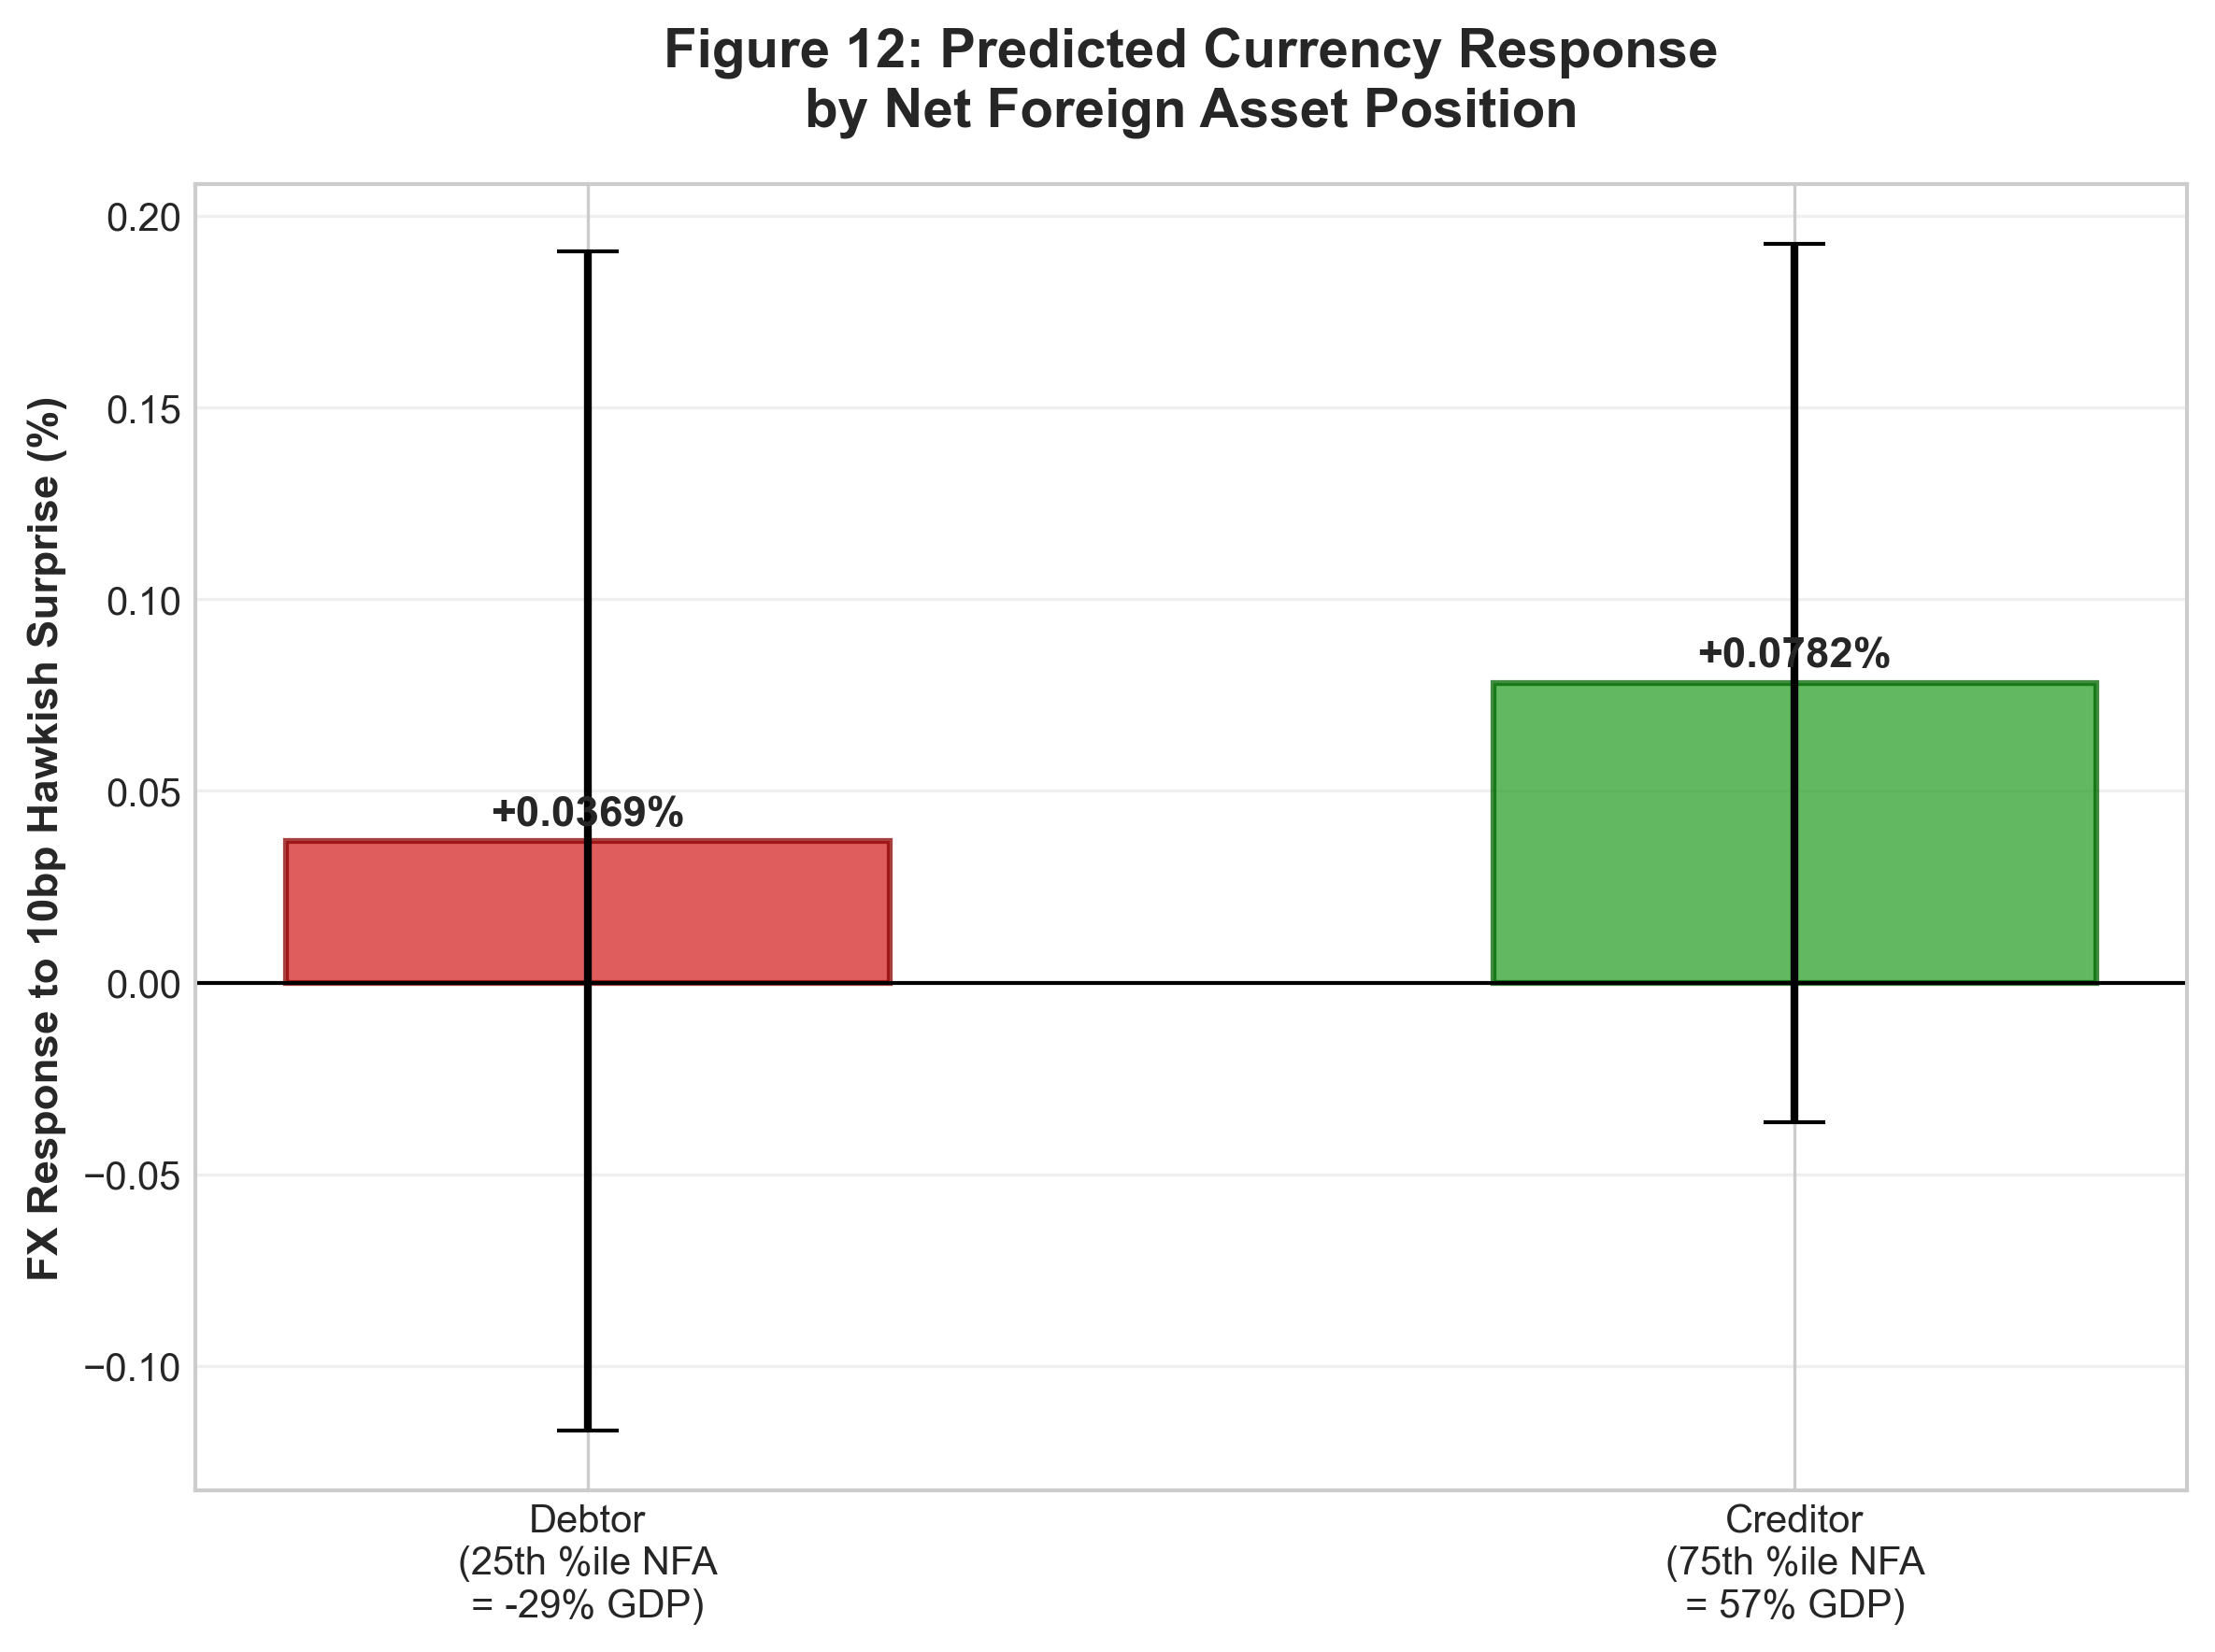
\includegraphics[width=0.85\textwidth]{figure12_predicted_responses.png}
\caption{\textbf{Economic Magnitude: Debtor vs Creditor Response.} Implied FX response for P25 (debtor) vs P75 (creditor) to 10bp shock. Difference is economically modest and statistically insignificant.}
\label{fig:debtor_creditor}
\end{figure}

\begin{figure}
\centering
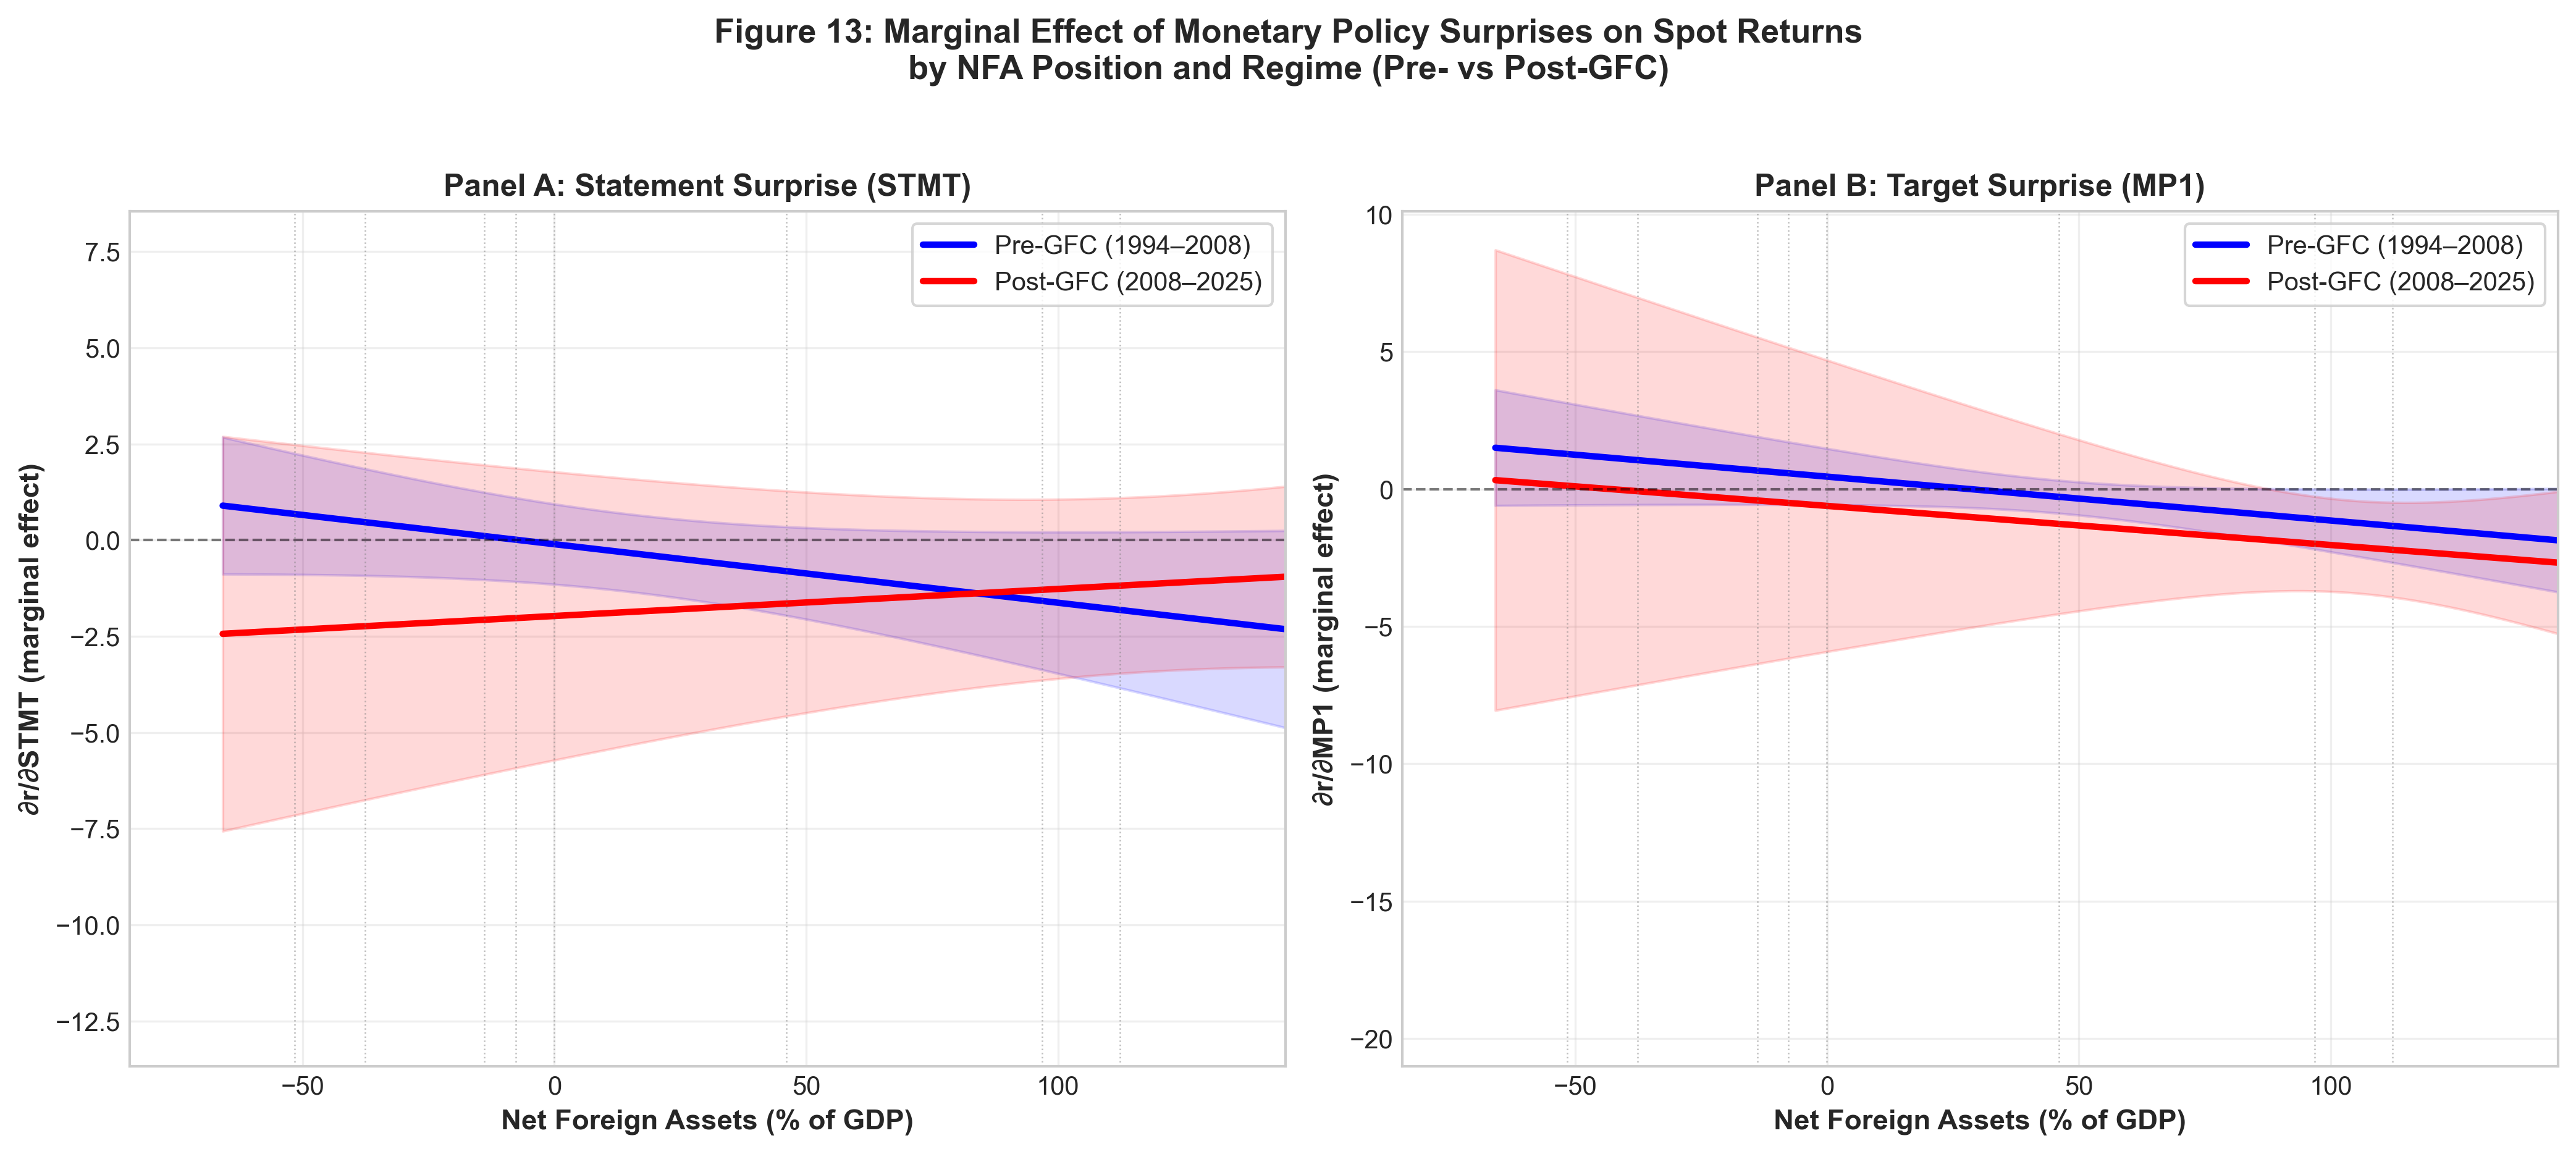
\includegraphics[width=0.9\textwidth]{figure13_time_variation.png}
\caption{\textbf{Marginal Effects by Regime: Pre- vs Post-GFC.} Lines are not statistically distinguishable, indicating little evidence of post-GFC amplification.}
\label{fig:time_variation_marginal}
\end{figure}

\begin{figure}
\centering
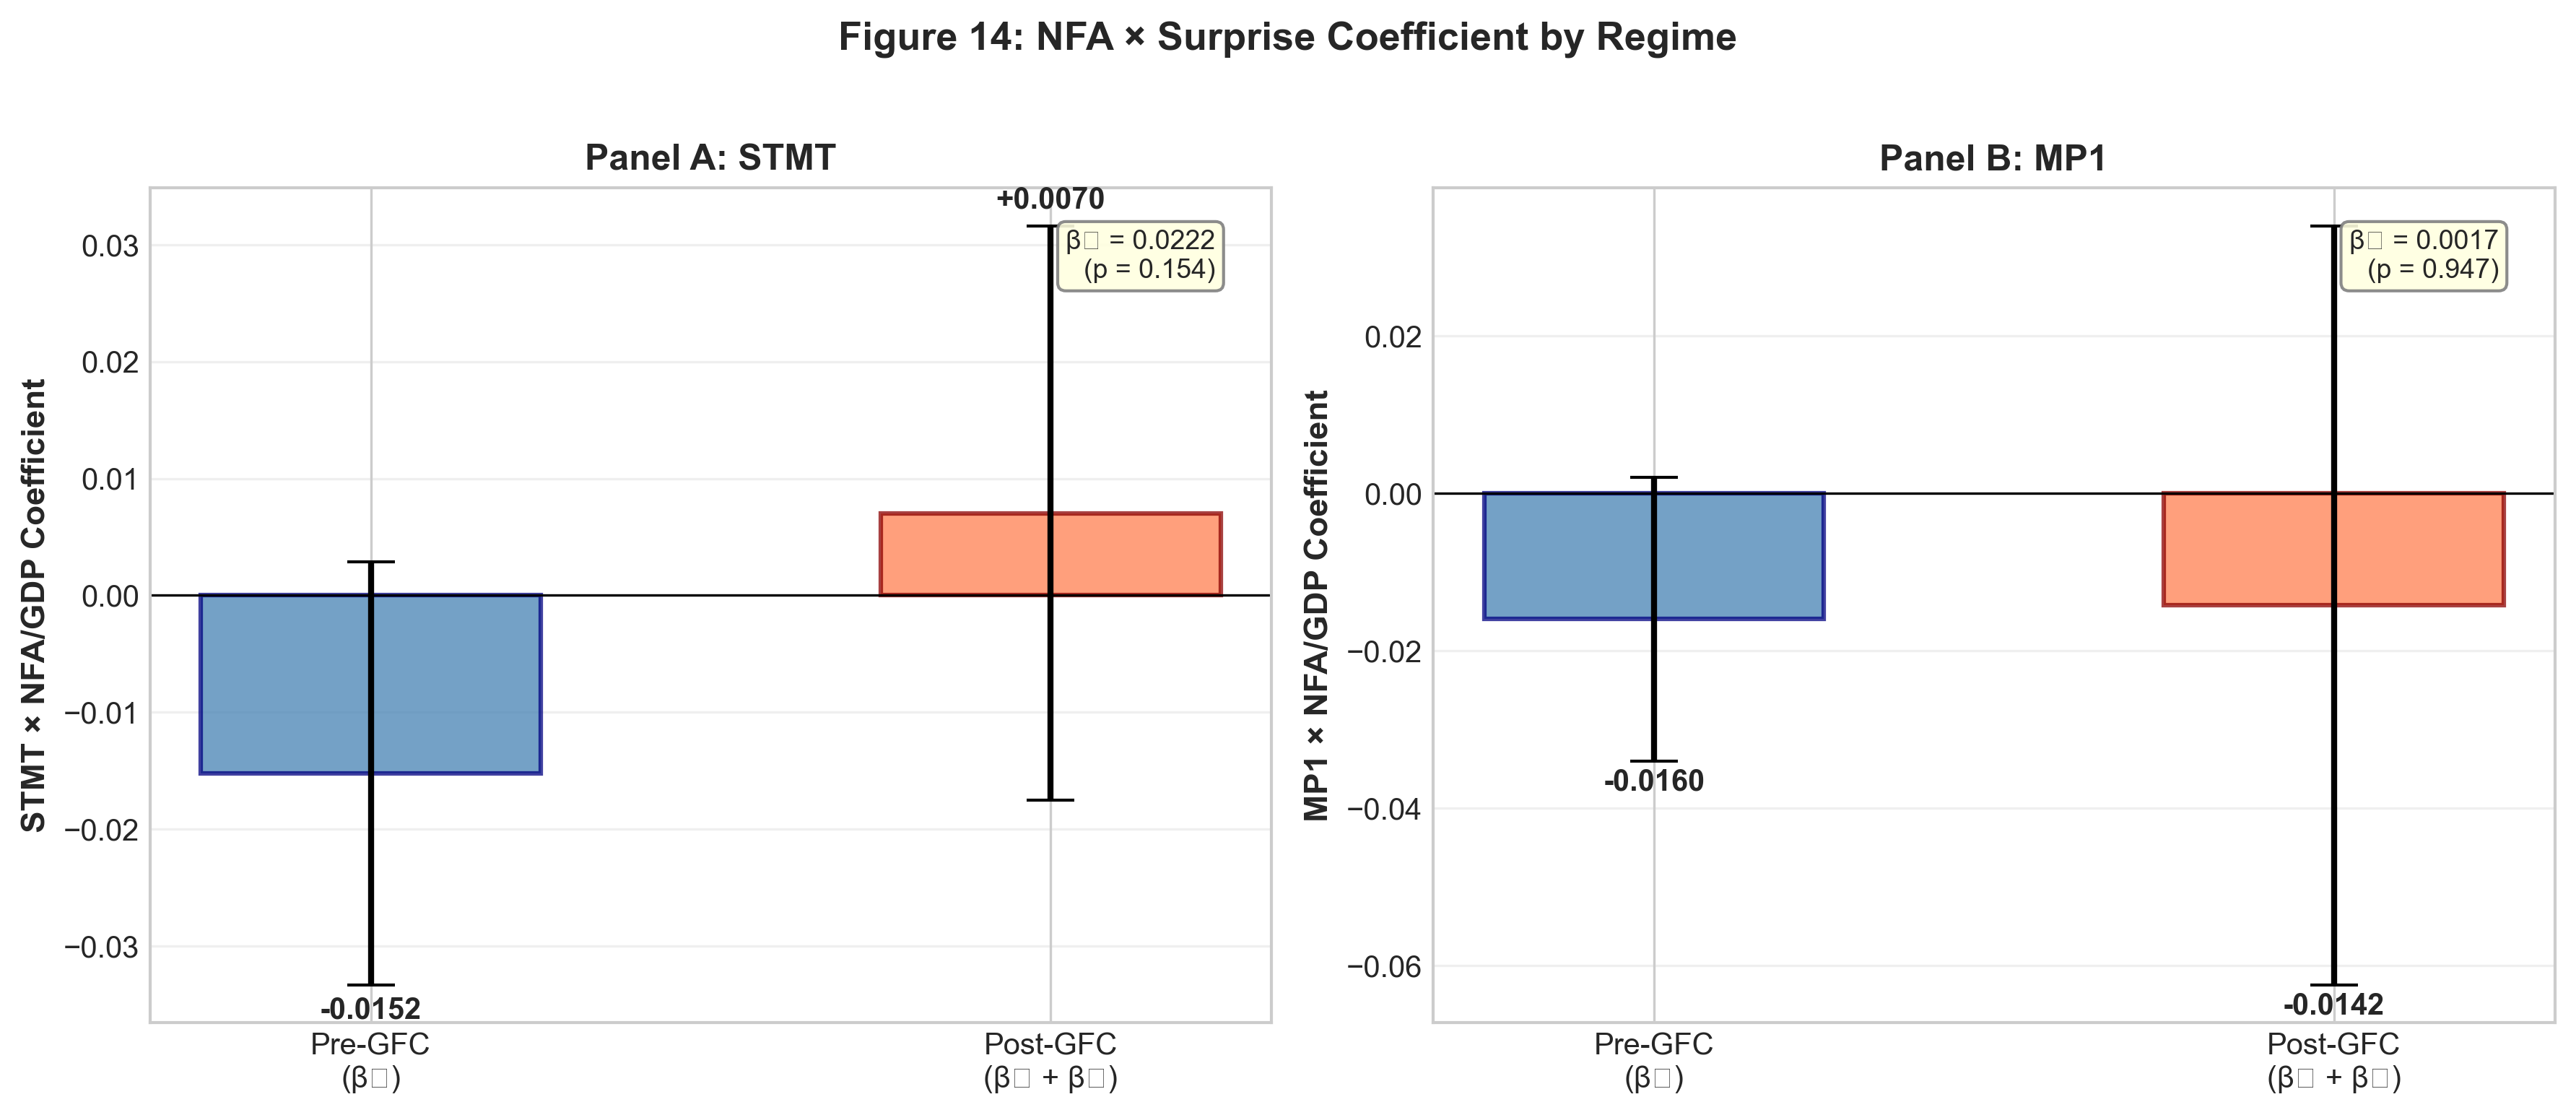
\includegraphics[width=0.85\textwidth]{figure14_coefficient_comparison.png}
\caption{\textbf{NFA Slope Pre- vs Post-GFC.} The ``post-GFC amplification'' term ($\beta_3$) is not precisely estimated.}
\label{fig:time_variation_coef}
\end{figure}

\begin{figure}
\centering
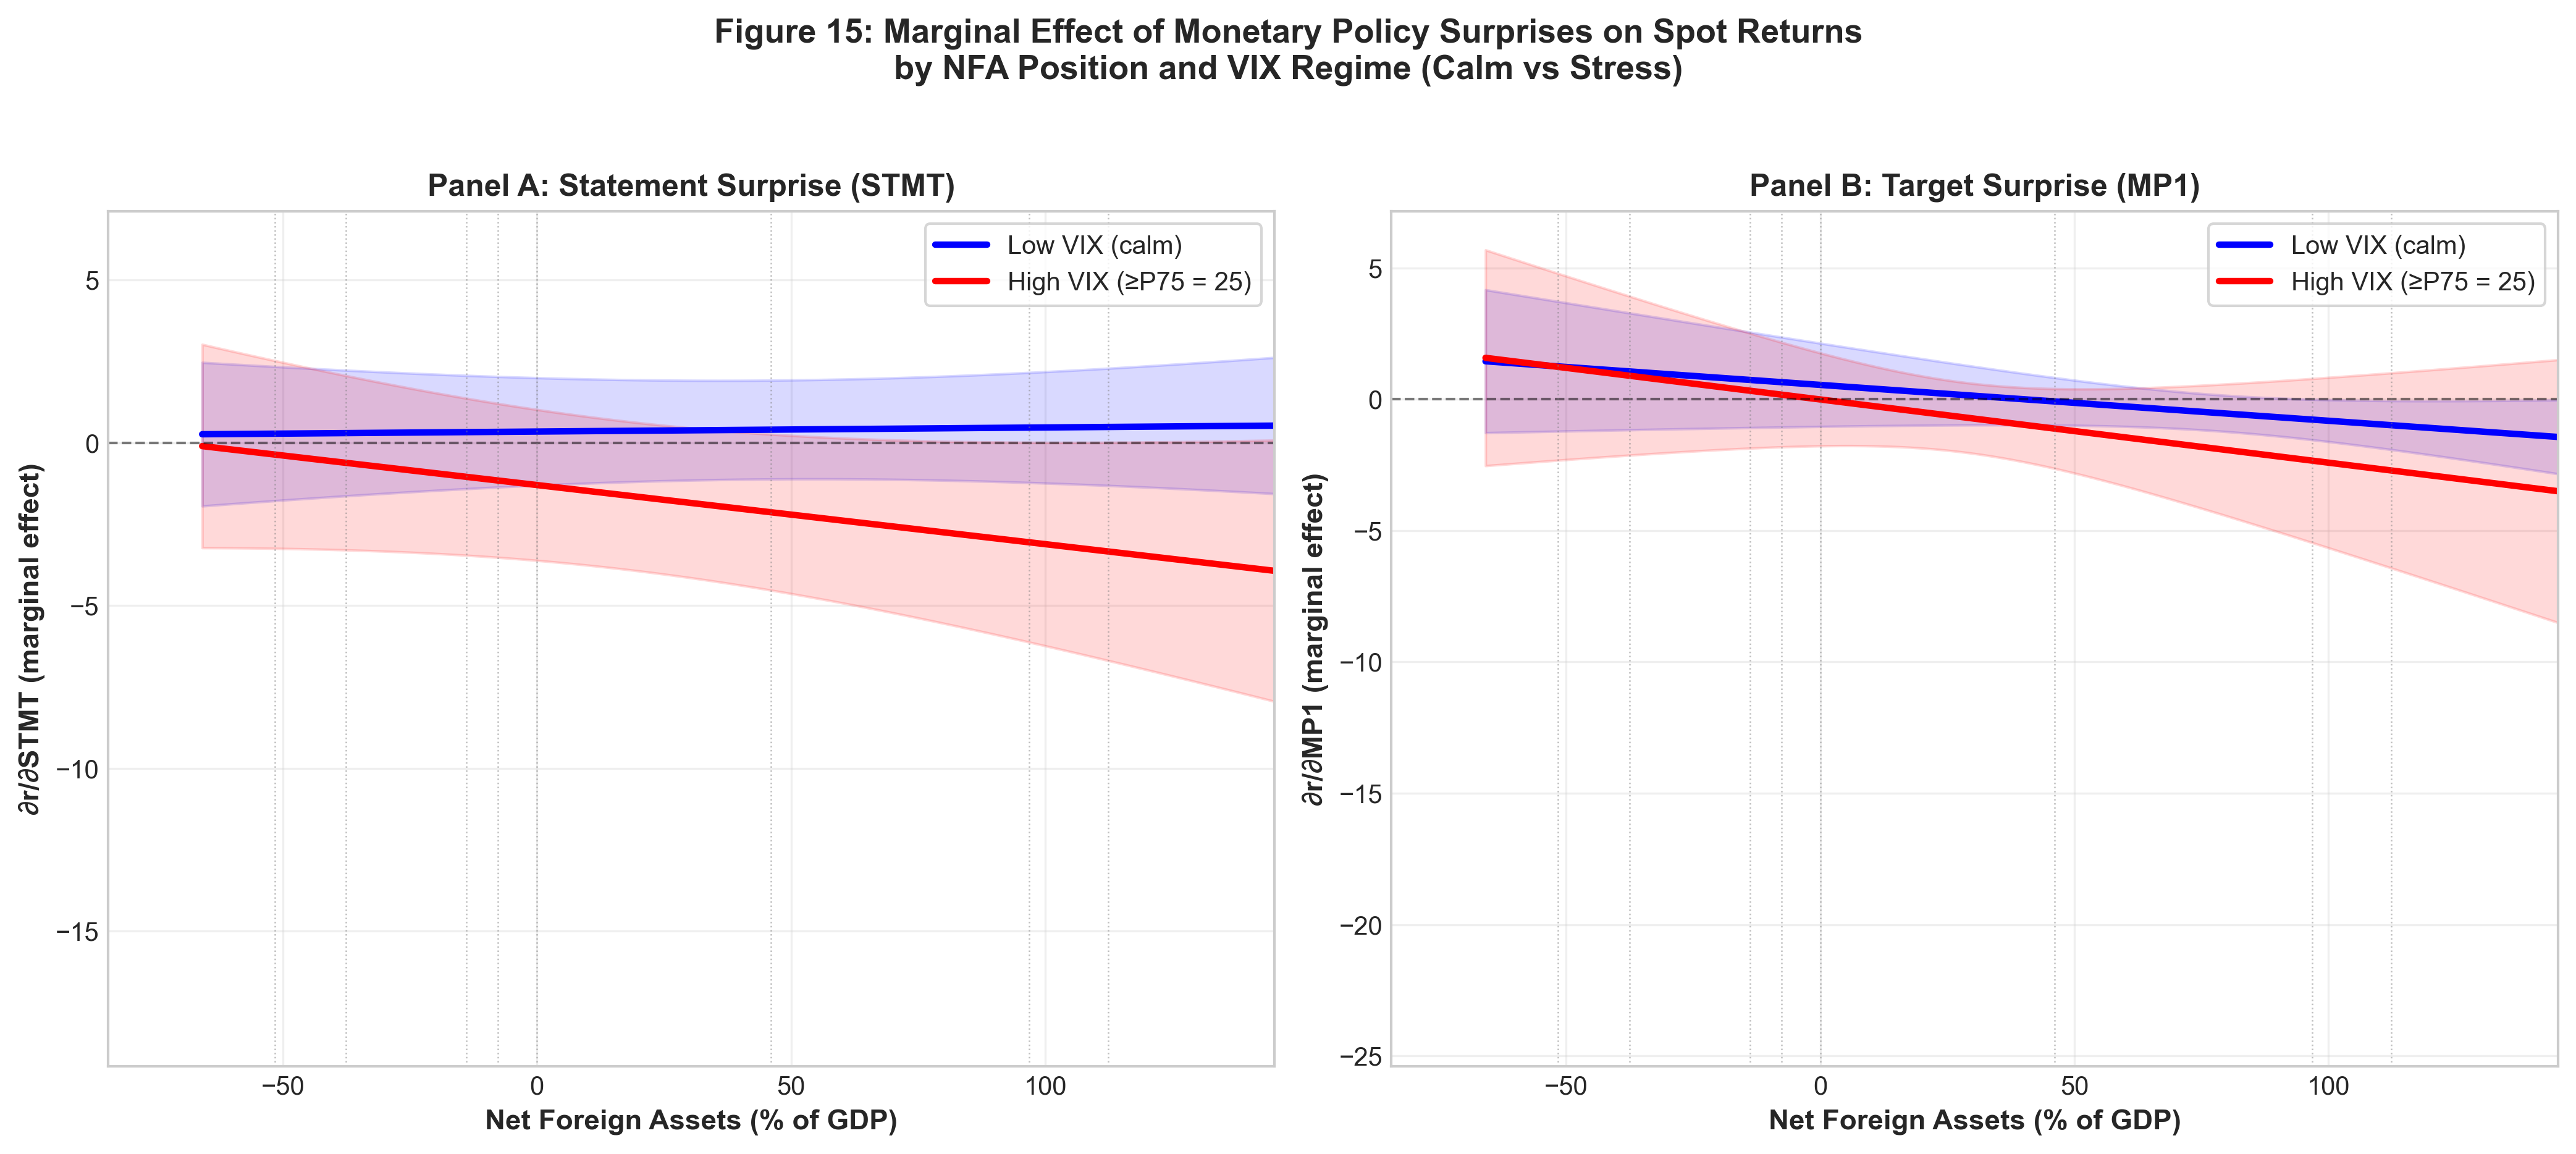
\includegraphics[width=0.9\textwidth]{figure15_vix_stress.png}
\caption{\textbf{Marginal Effects by VIX Regime.} The NFA slope does not reliably steepen in high-VIX periods.}
\label{fig:vix_marginal}
\end{figure}

\begin{figure}
\centering
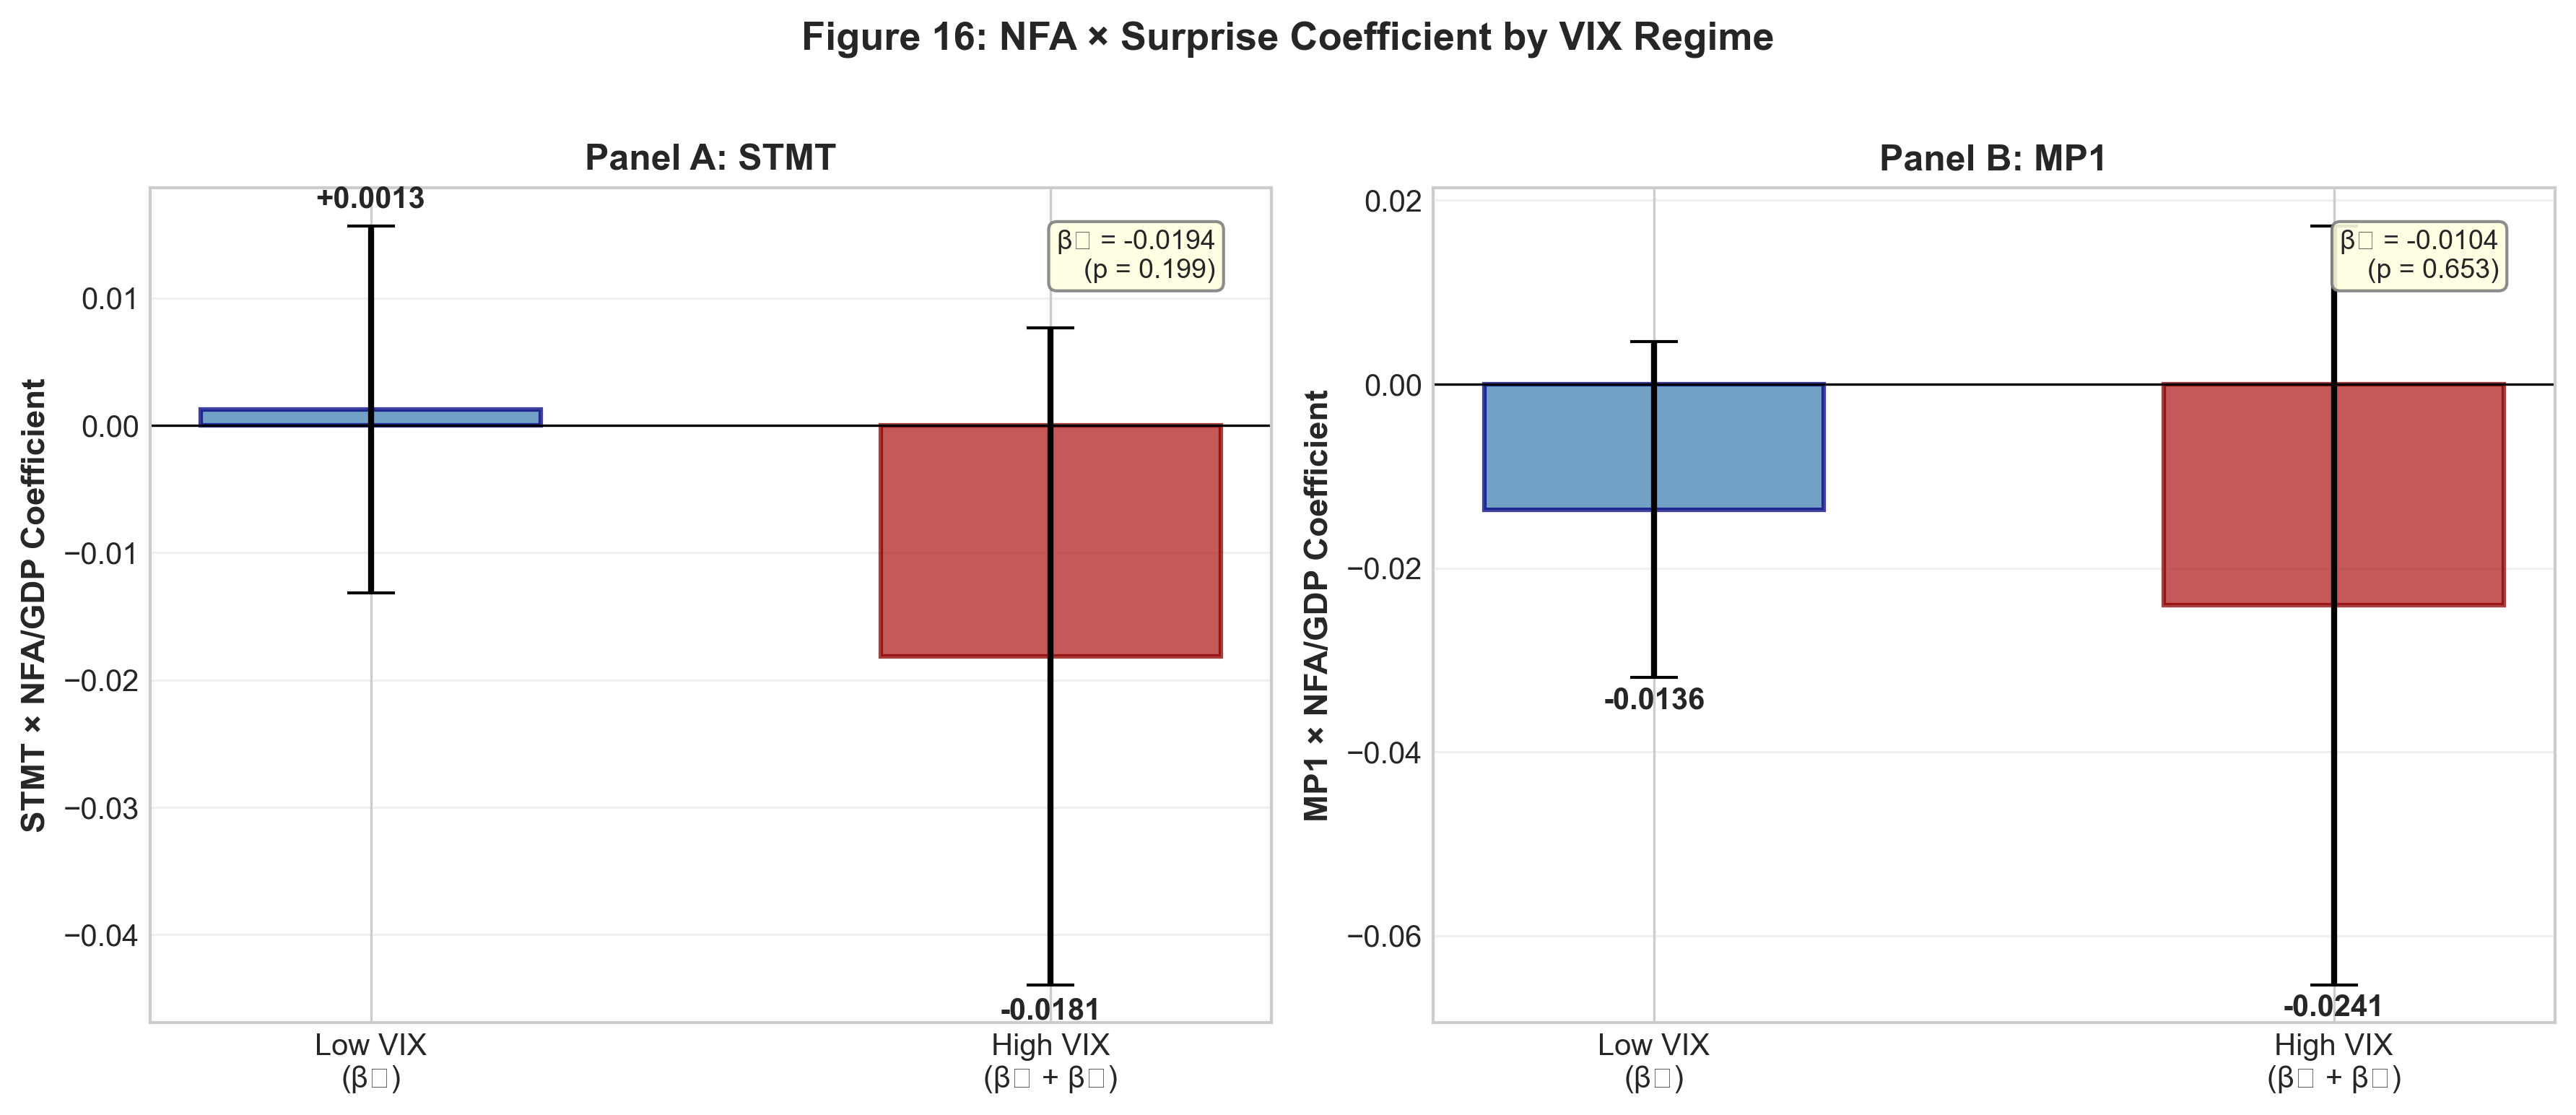
\includegraphics[width=0.85\textwidth]{figure16_vix_coefficient_comparison.png}
\caption{\textbf{NFA Slope: Calm vs Stress Regimes.} The stress-state amplification term is indistinguishable from zero.}
\label{fig:vix_coef}
\end{figure}

\end{document}
